\documentclass[12pt,oneside,justify,table]{book}

\usepackage[utf8]{inputenc}
\usepackage{mathptmx}
\usepackage{geometry}
\usepackage{fancyhdr}
\usepackage{tocloft}
\usepackage{titlesec}
\usepackage{textcomp}
\usepackage{pdfpages} 
\usepackage{graphicx}
\usepackage[magyar]{babel}
\usepackage{t1enc}
\usepackage{indentfirst}
\usepackage[shortcuts]{extdash}
\usepackage[toc,page]{appendix}
\usepackage{tabularx}
\usepackage{float}
\graphicspath{ {images/} }
\usepackage[backend=biber,]{biblatex}  % irodalomjegyzék

\titleformat{\chapter}{\normalfont\huge}{\thechapter.}{20pt}{\huge} % egyedi chapter szöveg

\geometry{
	a4paper,
	lmargin=3cm,
	tmargin=3cm,
	bmargin=3cm,
	rmargin=2cm
}

\fancyhead
\fancyfoot
\pagestyle{plain} % oldalstílus
\pagenumbering{arabic} % oldalszámozás 

\renewcommand{\headrulewidth}{0pt}
\renewcommand{\contentsname}{Tartalomjegyzék} % tartalomjegyzék átnevezés
\renewcommand{\listfigurename}{Ábrajegyzék} % ábrajegyzék átnevezés
\renewcommand\cftchapaftersnum{.} % chapter szám utáni pont
\renewcommand\cftchapdotsep{\cftdotsep} % chapter és irodalomjegyzék szöveg utáni pontok
%\newcommand{\sectionbreak}{\clearpage} % címsorok új oldalon
\renewcommand{\appendixname}{Függelék} % Függelék sor átnevezés
\renewcommand{\appendixpagename}{Függelék} % Függelék oldal átnevezés
\renewcommand{\appendixtocname}{Függelék} % Függelék tartalomjegyzék bejegyzés átnevezése

\addbibresource{bibliography.bib}

% help section - to be deleted

% \chapter{Második bekezdés}
% \section{másik bekezdés 2 szintű}
% \subsection{First Subsection}
% \paragraph{az}

% Ezt idéztem \cite{AzureFundamentals}

% \noindent // bekezdés első sorának  nem indentálása

% end help section

\begin{document} 

\includepdf{outer_cover.pdf}
\includepdf{inner_cover.pdf}

\tableofcontents

\chapter{Virtualizációról}

A számítógépek már a kezdetekben is annyira erősek voltak, hogy átlagos felhasználási módokkal nem lehetett teljesen kihasználni a számítási teljesítményt vagy a tárkapacitást.
Ennek a problémakörnek a megoldására az igény az 1960-as évek közepén kezdett megnövekedni. 
Az akkori rendszerek single user, single application módban voltak képesek működni. 
Ez annyit tett, hogy a felhasználónak, ha egyszerre több folyamat futtatására volt szüksége, akkor annyi számítógépet kellett üzemeltetnie. 
A két éllovas az MIT és az IBM volt, az első kész megoldást azonban az IBM szállította. 
Az MIT-n akkor nem jól mérték fel a feladat jelentőségét, így nem szenteltek neki kellő figyelmet és elvesztették vezető szerepüket. 
Az IBM megoldásában egy specializált mainframe rendszert használtak, ahol a felhasználók párhuzamosan tudták futtatni a saját programjaikat.
A felügyeletre pedig egy parancssor állt rendelkezésre.
Ez azért volt nagy előre lépés, mert így a felhasználók egymástól elszeparált módon dolgozhattak.
Ez volt az első lépcső a virtualizáció mai formája felé.

A virtualizáció nem csupán az optimálisabb erőforrás elosztáshoz volt szükséges. 
A minden folyamatra külön kiszolgáló fenntartása komoly feladatok elé állította az üzemeltetésüket végzőket. 
A szerverek magas száma miatt nagy méretű adaközpontokat kell építeni, amelyekben a megfelelő körülmények fenntartása nagyon költséges. 
A sok különböző szerver üzemeltetése, adminisztratív szempontból sem kisebb feladat. 
A kezdeti rendszereket nem lehetett távolról egyszerűen vezérelni. Léteztek ugyan KVM megoldások amelyekkel limitáltan el lehetett végezni a távoli vezérlés bizonyos lépéseit, de például már a telepítéshez - főleg ha annak fizikai adathordozóról kellett megtörténni - szükséges volt a fizikai hozzáférés. 
A virtualizációs megoldások terjedésének köszönhetően, össze lehet fogni nagyobb csoportokba a szervereket. 
Aztán ezek felett a csoportok felett lehet definiálni az úgynevezett virtuális gépeket, amelyek osztoznak az erőforrásokon és a virtualizációs megoldástól függően akár mozoghatnak is a fizikai gépek között úgy, hogy a munkafolyamat nem szakad meg.

A fejlesztések azonban nem álltak le és megindultak a kutatások az alkalmazás virtualizáció irányába. 
Ezen irányú törekvések eredménye lett az egykori Sun Microsystems nevet viselő vállalat fejlesztése a Java. 
A Java nyelv legnagyobb előnye és egyben hátranya is, hogy bármely gépen elfut amelyen van Java Runtime Environment (JRE). 
A JRE felel azért, hogy az alkalmazások egy külön virtuális gépben fussanak az operációs rendszeren belül. 
Így az univerzális nyelven megírt alkalmazások teljesen szeparált, de előre jól tervezhető módon futnak szinte bármilyen hardveren és operációs rendszeren.

Jelenleg a virtualizációs megoldásokat már a biztonság fokozására használják, ezt bővebben a gyártóspecifikus részben taglalom.

\section{On-Premises rendszerek}
\noindent On-Presmises rendszerek esetén megjegyezném, hogy VMware és Hyper-V esetén a hardveres megkötései megegyeznek 2016-tól. \cite{VMwareLimits} \cite{Hyper-VLimits}\\

\noindent Gazdagépek tekintetében: \\
\begin{table}[ht]
\centering
	\begin{tabular}{l | l}
		\textbf{Összetevő} & \textbf{Limitáció} \\
		\hline
		Logikai processzorok & 512 db \\
		Memória & 24TB \\
		Futó virtuális gépek & 1024 db \\
		Cluster node-ok & 64 db \\
		Virtuális gépek a cluster-enként & 8000 db\\
	\end{tabular}
\end{table}

\noindent Virtuális gépeket illetően:
\begin{table}[ht]
\centering
	\begin{tabular}{l | l}
		\textbf{Összetevő} & \textbf{Limitáció} \\
		\hline
		Logikai processzorok & 240 db \\
		Memória & 12TB \\
		Virtuális Fibre Channel HBA & 4 db \\
		Virtuális SCSI kontroller & 4 db \\
		Virtuális SCSI lemez & 256 db összesen, 64 db kontrollerenként \\
		Virtuális hálózati adapter & 12 db \\
	\end{tabular}
\end{table}



\subsection{Microsoft Hyper-V\texttrademark}

A Microsoft Hyper-V története egészen 1997-ig nyúlik vissza, amikor is még a technológiát a Connectix nevű cég birtokolta. 
Az első verziós kiadása a Virtual PC-nek még Macintosh platformra készült el. 
Ezt követte 2001-ben az első Windowsos megjelenés. 
A Microsoft, miután egyértelművé vált, hogy az üzleti felhasználóknak szükségük van virtualizációs megoldásokra 2003-ban megvásárolta a Virtual PC-t és az akkor még nem kiadott Virtual Servert a Connectix-től. 
A Microsoft folytatta mindkét termék fejlesztését. A Virtual PC több frissítésen is átesett mígnem a Hyper-V le nem váltotta 2008-ban. 
A Virtual Server a kezdetektől fogva a szerver operiációs rendszerek és az üzleti felhasználók igényeinek megfelelően lett fejlesztve. 
Olyan nem elhanyagolható különbségekkel, hogy a szerver verzión már a kezdetektől fogva az NTFS akkori szabványának megfelelő 2TB-os méretet ki lehetett használni, míg a Virtual PC-n 127GB volt a maximum. 
A 127GB-os limit a korabeli merevlemezek kialakításából adódott, hiszen a konszumer lemezekben nem volt kontroller így az operációs rendszer nem cellák alapján címezte a lemezt hanem a geometriáját felhasználva, térben írta le a helyet. Ezt kellett használnia a virtuális lemezeknél is a VPC-nek, hogy az operációs rendszerek működőképesek maradhassanak.

A Microsoft Hyper-V ezen a néven először a Windows Server 2008 operációs rendszerben debütált. 
Megjelent belőle ugyanekkor egy ingyenes verzió is Hyper-V Server néven, amely nem volt más mint egy Windows Server 2008 Core edition, a Hyper-V role-al előtelepítve, míg a többi Role letiltásra került.
A Hyper-V most már minden mai Windows kiadásban rendelkezésre áll. A kezdeti limitált képességeit az újabb verziókkal kibővítette és most már teljesen valós opció a többi nagy virtualizációs platform mellett. 

A későbbiekben bemutatom azon funkcióit amelyek a virtualizált rendszereknél elengedhetelenek és amelyeknek köszönhetően a stabilitás, biztonság és a skálázhatóság megoldható a Microsoft saját rendszerével anélkül, hogy azok megvásárolható opciók lennének, mint más gyártóknál.

\subsubsection{Nano Server}

A Windows Server 2016-os kiadásával debütált és legfőbb célja a minimális overhead melletti üzemeltetés. 
Ezen kiadás telepítés utáni összmérete 800MB, grafikus felhasználói felülete nincs, mert távoli managementre lett tervezve.
A kis mérete miatt nagyon gyorsan telepíthető, kevesebbszer kell patchelni, a szokásos havi iterációk helyett negyedéves ütemezéssel. 
Ezzel a rendelkezésre állása megnőtt. 
Ugyan korlátozott funkciókra használható, de azokon a területeken nagyon fontos előrelépés. 
Nano Server lehet 
\begin{itemize}
	\item Compute Node egy cluster-ben
	\item Scale-Out file serverben Storage Host
	\item DNS szerver
	\item IIS Webszerver
	\item Containerben futó alkalmazás gazdagép
\end{itemize}

\subsubsection{Deduplikáció}

A Microsoft, a Windows Server 2012 szerver verzióban jelentette be a deduplikációt. 
A deduplikáció az a folyamat amely feldolgozza az engedélyezett lemezek tartalmát és egyező adatblokkokat csak egyszer tárol le. Az ismétlődő blokkok esetén már csak referenciákat, úgynevezett újraelemzési pontokat hagy. 
Ezzel a megoldással nagyon jó hatásfokkal lehet tárolóhelyet megtakarítani. 
A legjobban deduplikálható adatok a Virtualised Desktop Infrastructure -- későbbiekben VDI rendszerek -- amelyek esetén az operációs rendszer, a hozzátartozó frissítési csomagok és a feltelepített alkalmazások alapfáljai többnyire minden rendszeren megegyeznek. 
Amennyiben a virtuális gépeken nagyon kevés egyedi fájl és telepített alkalmazás található úgy a deduplikációs ráta elérheti akár a 80\%\=/ot is, ahogy az a \ref{fig:deduplication_ratio}. ábrán is látható.

\begin{figure}[H]
\centering
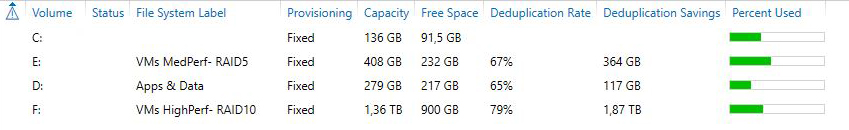
\includegraphics[width=1\textwidth]{deduplication-ratio-sample}
\caption{Deduplikációs ráta egy Hyper-V szerveren amelyen teszt szerverek futnak virtuális gépekként}
\label{fig:deduplication_ratio}
\end{figure}

\subsubsection{Cluster Rolling Upgrades}

A cluster-be fűzött hostokon futó operációs rendszert lecserélni nem volt egyszerű művelet, mert a Windows nem támogatta egy az egyben a frissítést. Így egy kerülő megoldást kellett használni az In-Place upgradehez. Egy ilyen folyamat a következő lépésekből áll:
\begin{enumerate}
	\item Egy node a régi cluster-ből való evakuálása.
	\item Az evakuált node újratelepítése az új operációs rendszerrel.
	\item A frissen telepített node\=/dal, egy gépből álló cluster létrehozása, a közös storage konfigurálása.
 	\item A virtuális gépek migrációja a két cluster között.

Mivel a Hyper-V nem támogat direkt cluster-to-cluster migrációt, ezért a virtuális gépeket először ki kell venni a magas rendelkezésre álló gépek közül. Ilyenkor azon a node\=/on tudnak csak létezni ahol akkor voltak, mikor megváltoztattuk a rendelkezésre állás szintjét.
	\begin{itemize}
		
		\item VM eltávolítása a magas rendelkezésre állású gépek közül
		\item VM migrációja az új cluster-re
		\item VM konfigurálása magas rendelkezésre állásúvá
	\end{itemize}
	\item Amikor már minden gépet lemozgattuk a következő telepítésre váró gazdagépről, akkor azt lehet újratelepíteni és hozzáadni az új cluster-hez.
	\item Amikor már csak egy node van a régi cluster-ben de már nincs rajta több virtuális gép, azt a cluster-t el kell pusztítani és a gépet újratelepítve be lehet kötni az új cluster-be.
\end{enumerate}

A Server 2016-ra történő frissítés során a cluster-ek lehetnek mixed módban. Azaz lehet bennük 2012 R2 és 2016-ot futtató host is. A mixed mód alatt a cluster a 2012 R2-es funkciókészletet használja, amikor befejeződik minden node\=/on a frissítés, onnantól használhatóvá válnak az új lehetőségek is. Az előzőekben taglaltam, hogy milyen lépések szükségesek ahhoz, hogy rolling upgrade nélkül el lehessen végezni a frissítést kiesés nélkül. 
Ugyanaz a folyamat rolling updrage használatával:
\begin{enumerate}
	\item A kiválaszott node\=/on találató VM-ek evakuálása.
	\item A node újratelepítése 2016-al.
	\item Az újratelepített node visszacsatlakoztatása a cluster-be. 
	\item Ugyanezen lépések ismétlése míg az utolsó node is újratelepítésre nem kerül.
\end{enumerate}

A 2016-ra való frissítést nagyon hamar fogják erőltetni az üzemeltetők, mert a 2016-os Hyper-V a virtuális gép leállítása nélkül képes a kiosztott virtuális processzor magok számának és az allokált memória mennyiségének növelésére és csökkentésére. Eddig ezekhez mindig le kellett állítani a guest gépet. 

\subsubsection{Scale-Out file server}

Világunkban a tárolandó adatmennyiség egyre csak növekszik. Léteznek olyan termékek melyek kimondottan csak az adattárolásra specifikálódtak pl. NetApp Appliances, DellEMC Compellent vagy XtremeIO rendszerek. Ezek nagy teljesítményt tudnak nyújtani az üzemeltetést segítő plusz funkciók mellett, ám ezek bekerülési költsége nagyon magas.
A Microsoft erre a feladatkörre fejlesztette ki a Storage Spaces technológiát és az arra épülő Scale-Out File Server\=/t.
\newline
A Storage Spaces technológia lényege, hogy sok, akár különböző lemezt tudjon összefogni egy logikai egységgé, amely fölött virtuális meghajtókat definiál. Ezen virtuális meghajtók nagyon hasonlítanak a RAID tömbök felett definiált meghajtókra, hiszen ugyanúgy meg kell adni a hibatűrését.  A Storage Spaces nagy előnye, hogy képes a virtuális meghajtókat több különböző típusú lemezből elkészíteni. Például létrehozhatunk SSD cache-l megtámogatott virtuális meghajtót, amely esetén az adatok mozgatását a rendszer végzi, az alkalmazások és a felhasználók számára teljesen transzparensen, hasonló módon mint ahogy az operációs rendszerek a memóriát lapozzák.

A Scale-Out File Server képessége, hogy 2 és 8 node közötti failover cluster-t hoz létre amelyen a megosztott meghajtók ugyanúgy működnek mint a Hyper-V Failover Cluster-ben a virtuális gépek. Tehát ha valamelyik storage node\=/ot le kell állítani akkor az ő által birtokolt megosztások átkerülnek egy másik node\=/ra, a lemezei vezérlését pedig szintén egy másik node veszi át.

\subsubsection{Storage Spaces Direct}

Windows Server 2016-al debütált megoldás, amely az alacsonyköltségvetésű cluster-ek kiépítését segíti elő. A Failover cluster-ek alap követelménye, hogy legyen egy közös tárolóhely ahol virtuális gépek lemezfáljai és a konfigurációs fáljuk tárolva van. Így amikor a virtuális gépet mozgatni kell a node\=/ok között akkor csak az aktuális memória állapotot kell átmásolni az új hostra és már mehet is tovább a munka. 
A Storage Spaces Direct lényege, hogy a hostok saját beépített lemezeiket használják. A rendszer majd később ezekből a lemezekből készít egy disk poolt és azon definiálhatóak a tényleges meghajtók. Ezek a meghajtók a kialakítás miatt hibatűrőek és az adatok úgy vannak elosztva, hogy a munkafolyamat akkor is tud tovább menni, ha az egyik cluster node leáll vagy leszakad a hálózatról.
A rendszer bármikor bővíthető mert a háttérben a SoFS adja a megoldást.

\subsubsection{Storage Replica}

Windows Server 2012R2-től elérhető funkció a Hyper-V replica. A replikációnak köszönhetően fenn lehet tartani egy teljesértékű másolatát egy virtuális gépnek vagy gépek halmazának. A replikációs intervallum 1 óra és 5 perc között konfigurálható, azaz ha az eredeti gép megáll vagy valamilyen probléma adódik vele, akkor a replikát el lehet indítani ezáltal maximum a konfigurált replikációs időtartamnyi munkafolyamat elvesztésével kell számolni. Ezzel a megoldással jól lehet Off-Site backup-okat készíteni, akár Azure Cloud-ba is.

A Storage Replica az Hyper-V Replica másolata, csak itt a SoFS meghajtóit lehet biztonságosan tükrözni egy másik példányra.

\subsubsection{Virtual Network}

A Hypervisor-ok már a kezdetektől fogva képesek voltak a virtuális hálózatok kezelésére. Továbbá képesek a saját fizikai hálózati portjukon keresztül több különböző forgalmat lebonyolítani, plusz a szerver rendszerekben rendelkezésre áll a fizikai hálózati kártyák egy csoportba való összefogása. Ekkor az átviteli sebességet nem tudjuk aggregálni, tehát hiába fogunk össze 4 db 10Gbps hálózati linket, nem tudunk egyszerre kifelé 40Gbps-el kommunikálni egy adott host felé. Azonban ha egy időben 4 különböző host-al szeretnénk a kommunikációt végre hajtani akkor az egyéni linkek maximális sebességét érhetjük el. 

A virtuális hálózatoknak köszönhetően a host-okon vagy cluster-eken belül tudunk privát alhálózatok létrehozni amellyel az adatközlést még biztonságosabbá és szeparáltá lehet tenni.

\subsection{VMware vSphere\textsuperscript{\textregistered}}
A VMware céget 1998-ban alapították. Eleinte csak operációs rendszeren belül nyújtottak virtualizációs megoldást a Workstation  termékvonallal. 2003-ban jelentették be az elhíresült hipervizorjukat az ESX-et, amely valójában egy rövidítése az Elastic Sky X szavaknak. Ezzel egyidőben megjelent a VMware VirtualCenter amely az ESX-el együtt a VMware Infrastructure nevet viselte. A vSphere nevet 2009-ben vette fel amikor is a VI 3.5 folytatása már az új néven lett bemutatva. Az évek folyamán a korai verziók felül emelkedtek az ellenfeleken szolgáltatás kínálatban, mert sok olyan funkciót tartalmaztak amelyeket a konkurensek nem tudtak. Ugyanakkor ezekért a funkciókért felárat kellett fizetni. Microsoft Server 2016-al bemutatkozott Hyper-V már mindenben ugyanazt kínálja, csak más néven. 2008-ban ugyan ingyenessé tették az ESXi hipervizort, viszont az ingyenes nem licenszelt termék komoly megkötésekkel üzemel csak.  \\

\subsubsection{ESXi}
Az ESXi úgynevezett egyes típusú hipervizor. Ez annyit jelent, hogy nem egy alkalmazás amely az operációs rendszer fölé húz egy réteget amelyben képes virtuális gépeket futtatni, hanem egy kernel, amely futtatja a VM konténereket. Fontos megjegyeznem, hogy a Hyper-V is ugyanígy működik annyi különbséggel, hogy a szerepkör aktiválódása után, az újrainduláskor az operációs rendszer futtatása is a Hyper-V alá kerül be. Az ESXi egyik nagy előnye volt a kis mérete (kb 110MB telepítve) és ebből adódóan a patchelések szükségességének a ritkasága is, azonban a Microsoft Nano Server megjelenése óta ebben sem különbözik. 

Az ESXi konzol képernyője ugyanúgy csak egy recovery console mint a Nano Server esetén, csak a legfontosabb beállításokat lehet innen elvégezni, minden másra ott a webfelület amelyet minden host futtat, vagy be lehet kötni vSphere konzolba. \\

\subsubsection{vSphere} 
A vSphere egy management tool amely az ESXi gazdagépeket és a VMware cloudban futó virtuális gépeket is képes kezelni. A 6.5-ös verzióval már ezek a szerverek is lehetnek cluster-ben így a központosított management felület mindig elérhető. Megjegyezném, hogy a Microsoft is rendelkezik egy ilyen termékkel amely a System Center csomag részét képező Virtual Machnie Manager. A VMM 2016 is már képes nagy rendelkezésre állású alkalmazásként futni. 

A vSphere elérhető webfelületen - amely a 6.5-ös verziótól HTML5 alapú, korábban Java alapokon nyugvott - vagy előtelepített alkalmazásból vSphere Client, de akár REST API-on keresztül is. A management további formáját képezi a PowerCLI amely a VMware rendszerekhez ad PowerShell interfészt.


\subsection{Oracle\textsuperscript{\textregistered} VM}
Nem maradhatott ki az üzleti felhasználásra szánt virtualizációs megoldásokból az Oracle sem. Ugyan történelme nem nyúlik vissza olyan régre mint a konkurenseké, hiszen 2007-ben jelentették be, de az alapját adó Xen hipervizor már jóideje piacon volt. Az Oracle megoldása abból a szempontból tekinthető különlegesnek, hogy ez az egyetlen olyan megoldás amely támogat SPARC alapú szervereket gazdagépként. Jól lehet ez nem olyan nagyon meglepő hiszen a SPARC processzorok is Oracle által alapított technológia. Azért állíthatják, hogy ők nyújtják a legjobban optimalizált megoldást, mert a processzortól az alkalmazásig mindenre van saját megoldásuk. Jó alternatíva lehet az OVM, mert ingyenes ahogyan a rajta futó operációs rendszer is. Megfelelően megválasztott alkalmazás szerver esetén ott sem jelentkezik licensz költség. Ugyanakkor azt fontos észben tartani, hogy mindez csak addig van így ameddig nincs szükség támogatásra. A támogatás ugyanis előfizetéses konstrukcióban érhető el és minden építőelemre külön meg kell vásárolni. 

\subsubsection{OVM} 
A Xen Project által fejlesztett nyílt forráskódú hipervizorra épül. Kiviteltől függően SPARC vagy x86-os platformon is képes üzemelni. Támogatott virtuális gépek tekintetében nincs eltérés: Linux, Windows és Oracle Solaris operációs rendszerek lehetnek. A hardveres limitációk terén itt vannak komolyabb eltérések: \cite{OVMLimits} \\
\begin{table}[H]
\centering
	\begin{tabularx}{\textwidth}{>{\hsize= .8\hsize}X | X | X}
		\textbf{Összetevő} & \textbf{Limitáció \newline OVM x86 esetén} & \textbf{Limitáció \newline OVM SPARC esetén}\\
		\hline
		Futó virtuális gépek & 2560 db \newline(10 VM/host, 256 szerver) & 32768 db \newline(128 VM/host, 256 szerver)\\
		Cluster node-ok & 32 db & 32 db \\
		Szerver csoport tagok \newline (nem cluster-ezett) & 64 db & 64 db \\
		Logikai processzorok & 288 (tesztelt) \newline 384 (elméleti) & Megegyezik a maximális mennyiséggel:\begin{itemize}
	\item SPARC M7-16: 4096 
	\item SPARC M6: 3072 
	\item SPARC M5: 1536
	\item SPARC T5: 1024
	\item Fujitsu M10: 2048
\end{itemize}\\
	\end{tabularx}
\end{table}

\subsubsection{Oracle VM Manager} 
Az Oracle megoldása a virtuális gépek és a cloudban található erőforrások menedzsmentjére. Amiben eltér a konkurensektől, hogy az Oracle tárolóegységeket is lehet ugyanebből a konzolból kezelni. 

\subsubsection{SPARC}
A SUN Microsystems által feljesztet RISC tipusú utasításkészlettel rendelkező processzorcsalád. 1984-ben kezdődött a fejlesztése, azonban sokáig license köteles megoldás volt. A SPARC International konzorcium a teljes architektúrát nyílttá tette, az egységesség és az elterjedés elősegítése érdekében. 1993-ban megjelent a 64 bites verziója is, azonban az elterjedésének nagy gátat szabott, hogy a korlátozott utasításkészlet miatt nehezebb volt fejleszteni rá. A jól skálázható architektúrája alkalmassá tette, hogy több szuperszámítógépet is építsenek SPARC processzorokra. 2011-ben készült el a Tokiói egyetem szuperszámítógépe amely az Oakleaf-FX nevet viseli. Ez a TOP500 18. helyét szerezte meg akkoriban az összesen 76800 processzor magjával. Az alapját az 1,848 GHz-es SPARC64 IXfx  16 magos processzorok adják. \cite{SPARC}

\section{Cloud megoldások}
A szolgáltató szerverek elhelyezésekor 3 nagy irányzatot lehet megkülönböztetni. Ezek a On-Premises, Private cloud és Public cloud. 

\subsubsection{On-Premises} 
A dolgozatom előző bekezdésében már leírtam a főbb on-premises szolgáltatókat és azok képességeit. A szervek a cég álltal birtokolt területen kerülnek elhelyezésre megfelelő körülmények fenntartására képes szerver szobákban. Minden hardver megvásárlásra vagy tartósbérletre kerül. Sok esetben az internet elérés és a bérelt vonalak költségei nagyon magasak. Napjainkban még ez a legelterjedtebb forma, azonban a magas bekerülési költség miatt egyre inkább más írányokban gondolkodnak az üzemeltetést végző csapatok.

\subsubsection{Private cloud}
A következő lépcsőfok a teljesen felhőből kiszolgált szolgáltatásrendszer irányában. Ebben az esetben a szerverek számára az ideális környezeti feltételek biztosítását valamilyen Adatközpont szolgáltatóra (pl. Equinix) bizzák. Ezt a lépcsőfokot sok cég azért alkalmazza, mert még nem állnak készen, hogy a jelenleg megépített rendszereiket átmozgassák a felhőbe. Léteznek olyan alkalmazások amelyeket nem éri meg kimozgatni, pl a nagy mennyiségű lokális rendszerekkel végzett kommunikáció miatt. További előnyökhöz felsorolható, hogy az adatközpontokból a minőségibb internet és bérelt vonal szolgáltatásokat helyiértékekkel alacsonyabb áron lehet beszerezni. Azoknak a cégeknek lehet érdemes ilyen rendszerek bérlésében gondolkodni, akik már rendelkeznek valamilyen cloud szolgáltatással, esetleg több kisméretű telephelyük van több országban. A globális bérelt vonal szolgáltatók jó megoldások lehetnek a globális nagyvállalatok számára. A legnagyobb hátrányuk az áruk. A globális szolgáltató intézi a helyi kis szolgáltatókkal a kommunkációt, és ennek meg is kérik az árát. Amennyiben nagy adatközpontoktól veszi a cég a nagysebességű bérelt vonalat, és a kisebb sebességűt megrendeli minden országban a helyi iroda IT személyzete, a költségeken nagy mértékben lehet faragni. \\
Private cloud egyik alfajaként felfoghatóak azok a rendszerek, amelyek valamely nagy felhőszolgáltató technikáját használják fel arra, hogy a saját telephelyen található szervereket menedzsmentjére. Ilyen megoldás az Azure Pack, vagy az azt leváltó Azure Stack. \\

\noindent \textbf{Azure Stack} \\
A Microsoft álltal nyújtott Azure Pack utóda. A rendszer lényege, hogy a System Center csomag Virtual Machine Manager  alkalmazásán keresztül menedzseli a kiszolgálókon futó virtuális gépeket eközben teljesen Azure szintű felhasználói élményt nyújtva. Egy nagyon egyszerű self-service megoldás, amelynek köszönhetően az üzemeltetést végző csapatok munkálya csökkenthető, hiszen a számítási kapacitást igénylő csapatok maguknak elkészíthetik a szükséges erőforrásaikat. A rendszer figyeli és tájékoztatja a felhasználót, hogy a rendelkezésre álló kapacitásból mennyit használt fel, illetve az előre meghatározott rendszertípusokból mennyit képes még elfuttatni a kiszolgáló. \\
Az Azure Stack hátránya, hogy csak a Microsoft álltal meghatározott és jóváhagyott hardverrel kompatibilis, amelyet egyenesen a partnerektől kell, hardver csomag - rack szekrény - formájában megvásárolni. A korlátozás azért szükséges, mert a rajta futó rendszer nagyban hasonlít ahhoz az egyedileg módosított Hyper-V szolgáltatáshoz ami az Azure-t is kiszolgálja. Az elterjedésében az előbb említett limitáció, nagyban hátráltatja. Az elődje nagy sikereket könyvelhetett el, mivel nem voltak ilyen szintű limitációk. 

\subsubsection{Public cloud}
Ez a legteljesebb megoldás. Ilyenkor a vállalat számára a telephelyekre csak megfelelő minőségű és sebességű internetet kell vásárolni, minden más rendszer a felhőben fut. Így megspórolható a kezdeti költségek közül a szerverszoba költségeit, és az azzal járó fenntartási költségeket. A felhő további előnye, hogy az igényeknek megfelelően módosítható a felhasznált számítási, tárolási kapacitás. Minden adat ami a felhőben áll elő, vagy oda feltöltésre kerül, annak a mentéséről a felhőszolgáltató gondoskodik, az előre közölt SLA-nak megfelelően. A magas rendelkezésreállás garantálására ugyanazt a szolgáltatás el lehet helyezni több adatközpontban, akár a világ több pontján is. Természetesen minden felhőben futó alkalmazás egymással magas sebességgel képes kommunikálni, hiszen az adatközpontok között megfelelő minőségű kapcsolat van kiépítve. Amint azt a továbbiakban látni lehet a \ref{fig:AzureRegions} és \ref{fig:AWSRegions} ábrákon, a felhő szolgáltatók is törekednek arra hogy ugyabban az országban, vagy városban települjenek le ahol a vetélytársak is, így nyújtva a legnagyobb sebességet. \\

Az elmúlt években érezhető a felhő felé fordulás, mert minden cégnek érdeke a költségek csökkentése és optimalizálása. Ezeket a kezdeményezéseket jól mutatják majd az \ref{fig:CloudTrends2018}-ös ábrán látható arányszámok. A két vezető felhőszolgáltató esetén már alacsonyabb a kisérletető cégek mennyisége, azonban a kisebb szolgáltatóknál ez még akár a felhasznált kapacitár harmadát is kiteheti. A Gartner által készített elemzés szerint 2021 lesz az az év, amikor megfordul az arány és a felhőből, vagy co-located szerverfarmokról lesznek kiszolgálva a rendszerek lásd \ref{fig:trends_gartner} ábra. 
\begin{figure}[H]
\centering
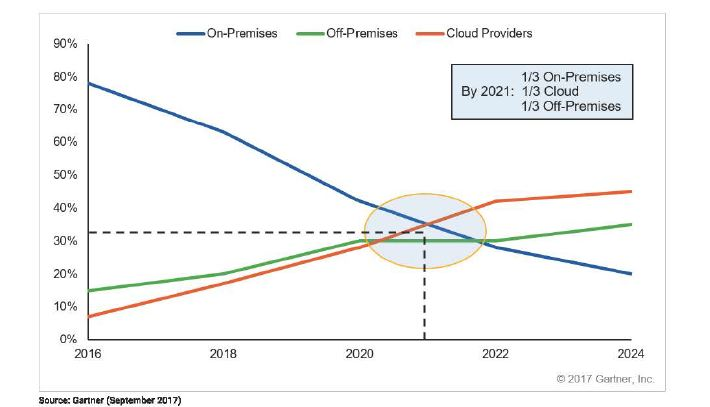
\includegraphics[width=1\textwidth]{trends_gartner.jpg}
\caption{Szolgáltatások kiszolálgálsi helye egymáshoz viszonítva, forrás: Gartner \cite{Gartner}}
\label{fig:trends_gartner}
\end{figure}

Az évek során jól láthatóan formálódott a vállalatok hozzáállása a felhőhöz. A \ref{fig:3yearCloudvsOnPrem} ábráról leolvasható, hogy az elmúlt 3 évben a private cloud megoldások felől, a public cloud irányába fordulnak a vállalatok.
\begin{figure}[H]
\centering
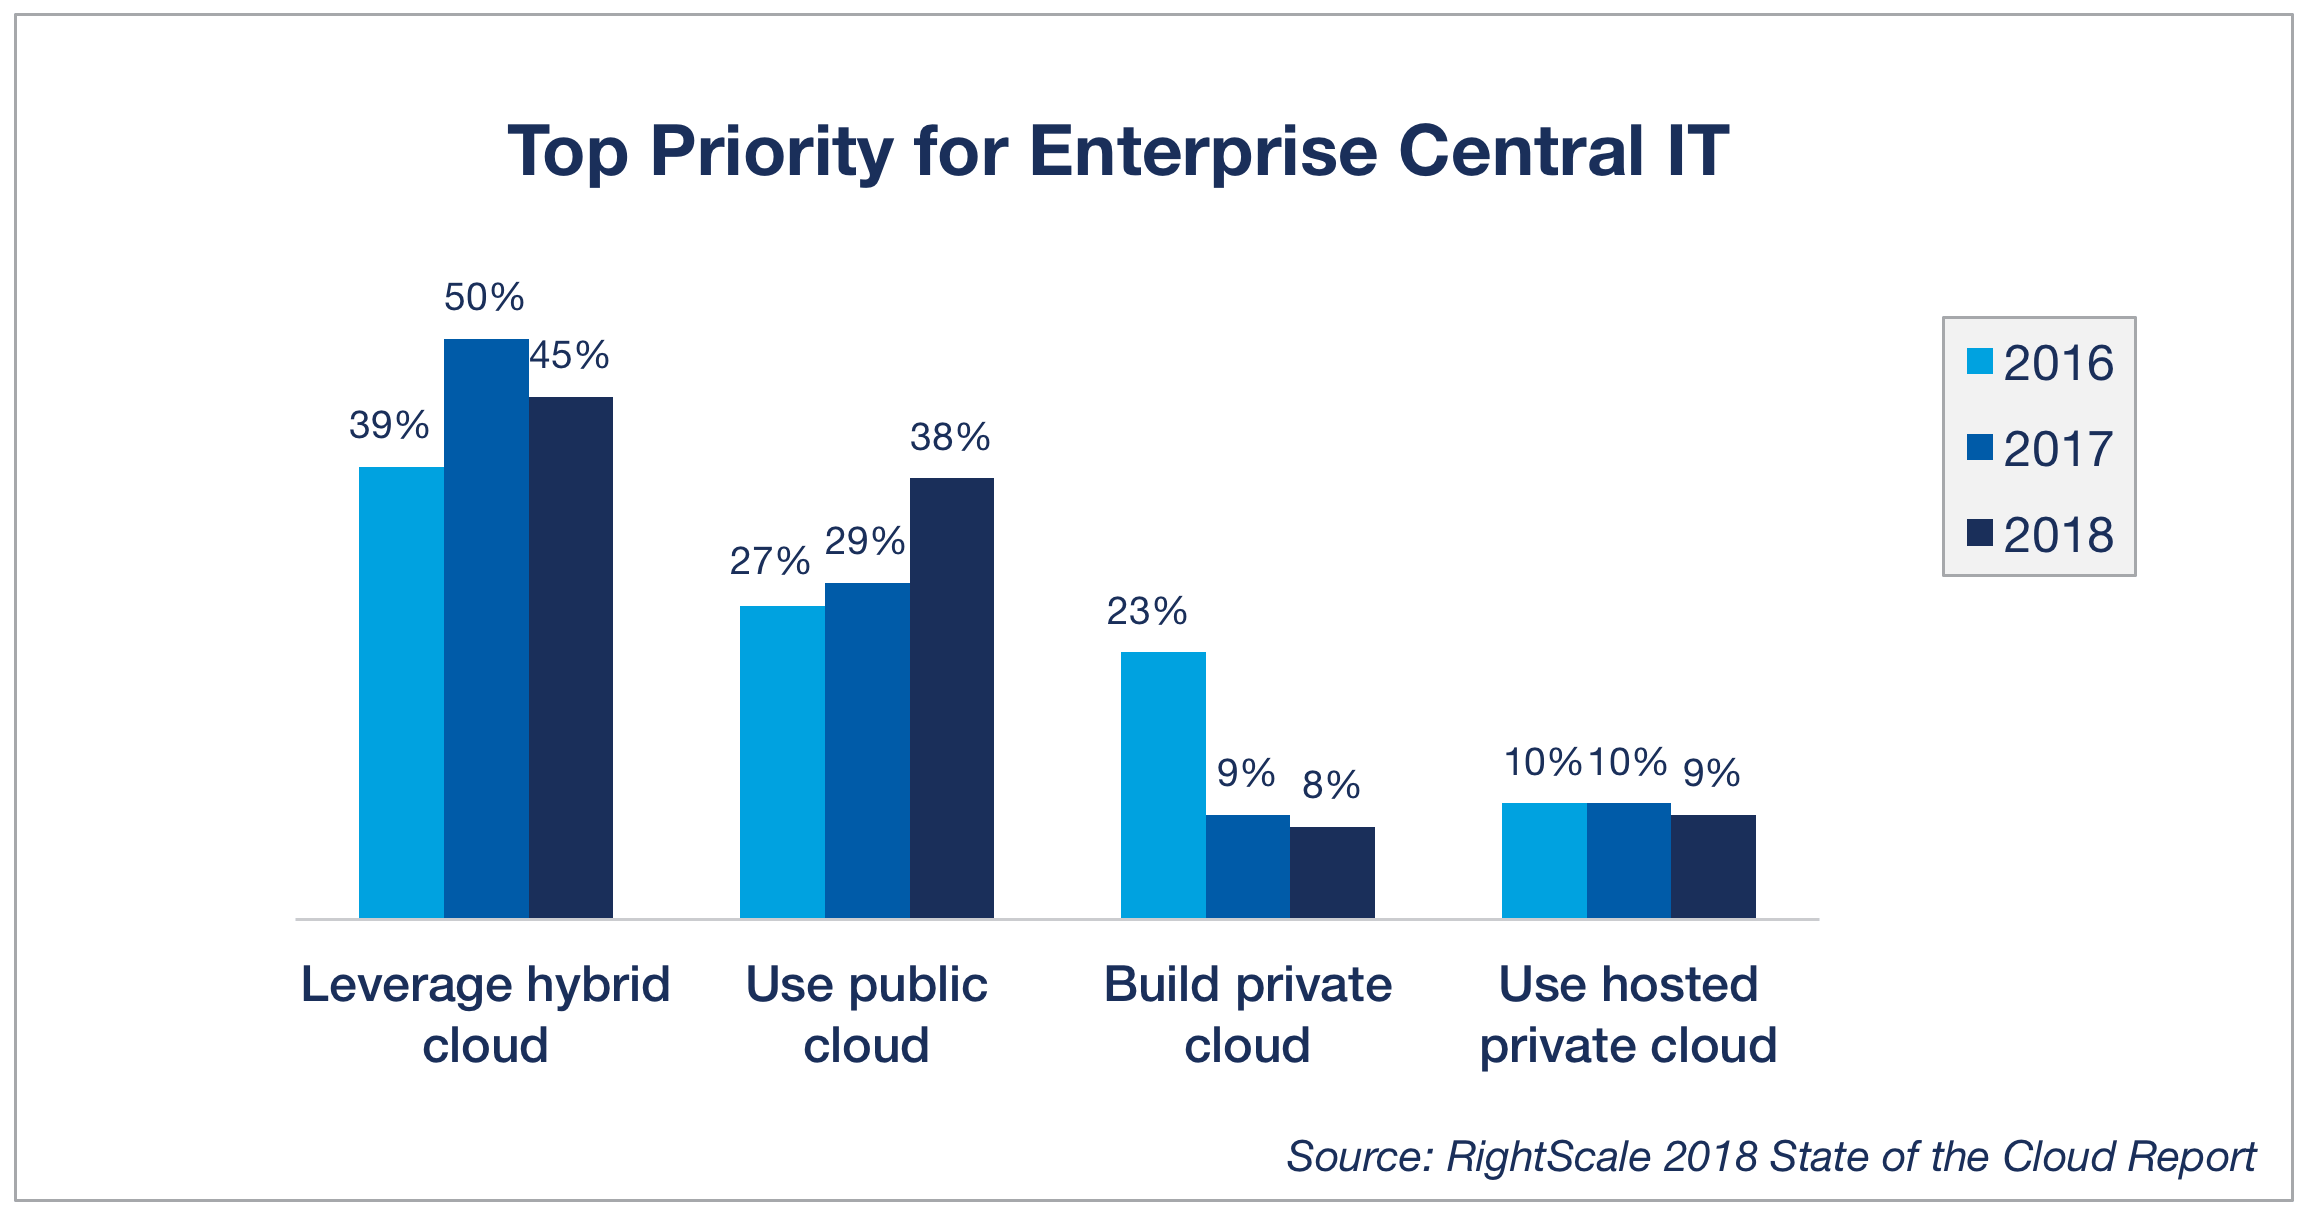
\includegraphics[width=1\textwidth]{4-Cloud-Computing-Trends-Enterprises-Prioritizing-Public-Cloud.png}
\caption{Szolgáltatás lokációk megoszlásának változása az elmúlt 3 évben, forrás: \cite{RightScale}}
\label{fig:3yearCloudvsOnPrem}
\end{figure}

Amielőtt a nagyobb felhő szolgáltatókról beszélnék, tanulságos lehet megvizsgálni a helyzetüket a piacon, lásd: \ref{fig:CloudAdoption2017-2018} ábra.
\begin{figure}[H]
\centering
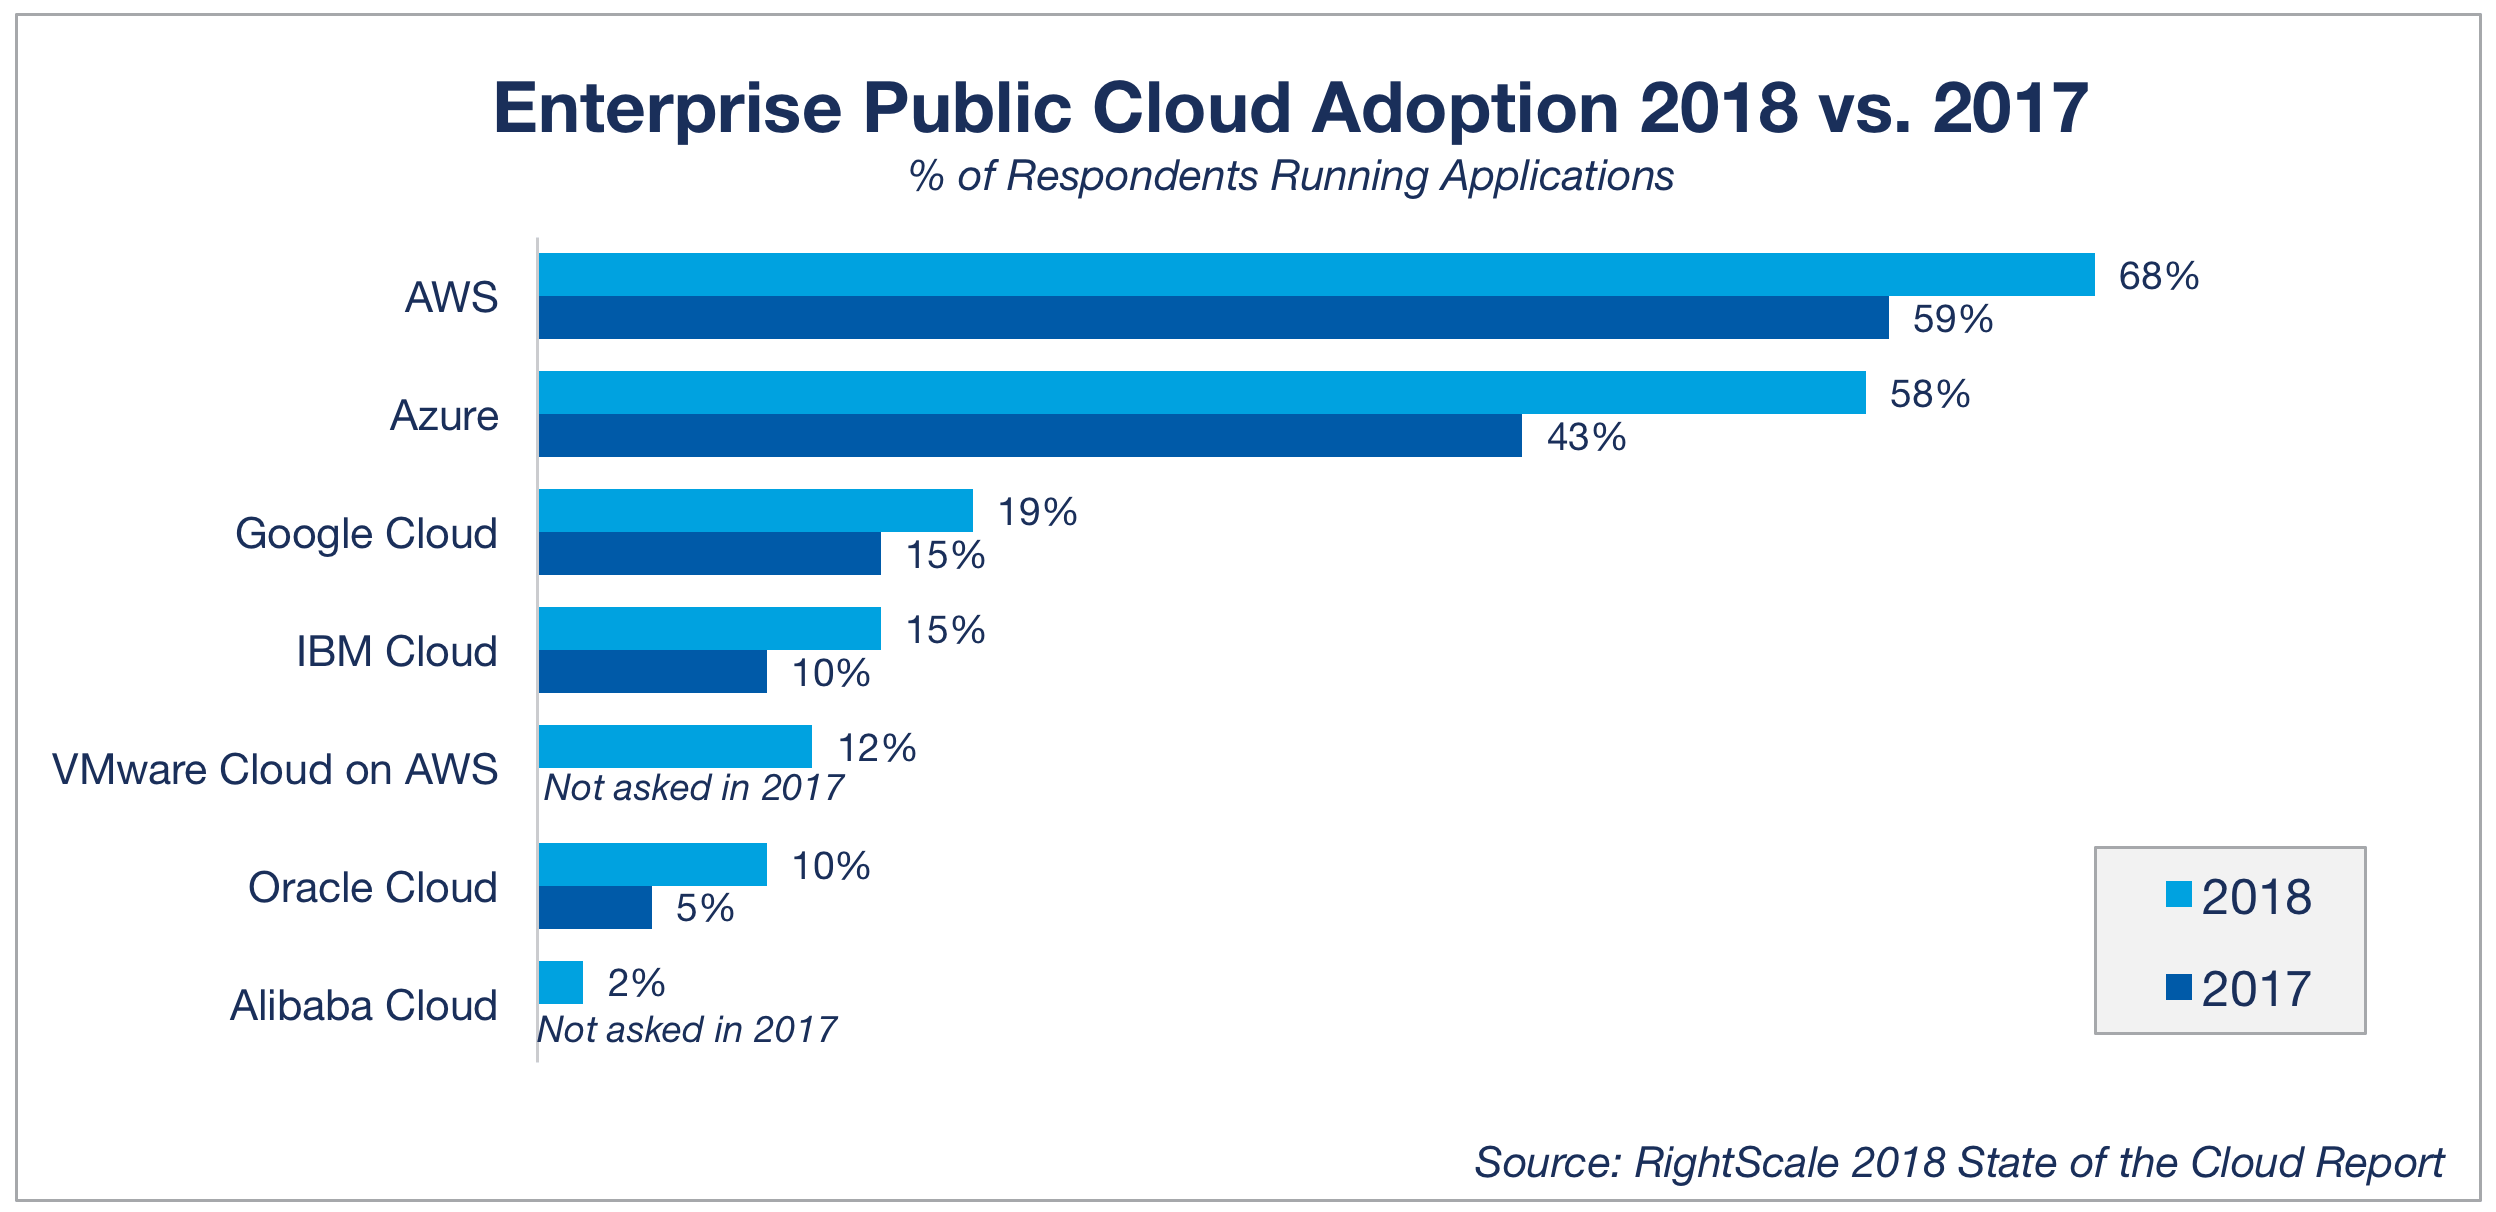
\includegraphics[width=1\textwidth]{22-Cloud-Computing-Trends-Enterprise-Public-Cloud-Adoption-2018-vs-2017.png}
\caption{Éves növekedése a platformok felhasználásának, forrás: \cite{RightScale}}
\label{fig:CloudAdoption2017-2018}
\end{figure}

A felhőben futó alkalmazások folyamatosan bővülnek, így érdekes viszonyszám, hogy mely platformon, mennyi a már beváltnak és stabilnak számító megoldás. Ezt mutatja a \ref{fig:CloudTrends2018} ábra. 
\begin{figure}[H]
\centering
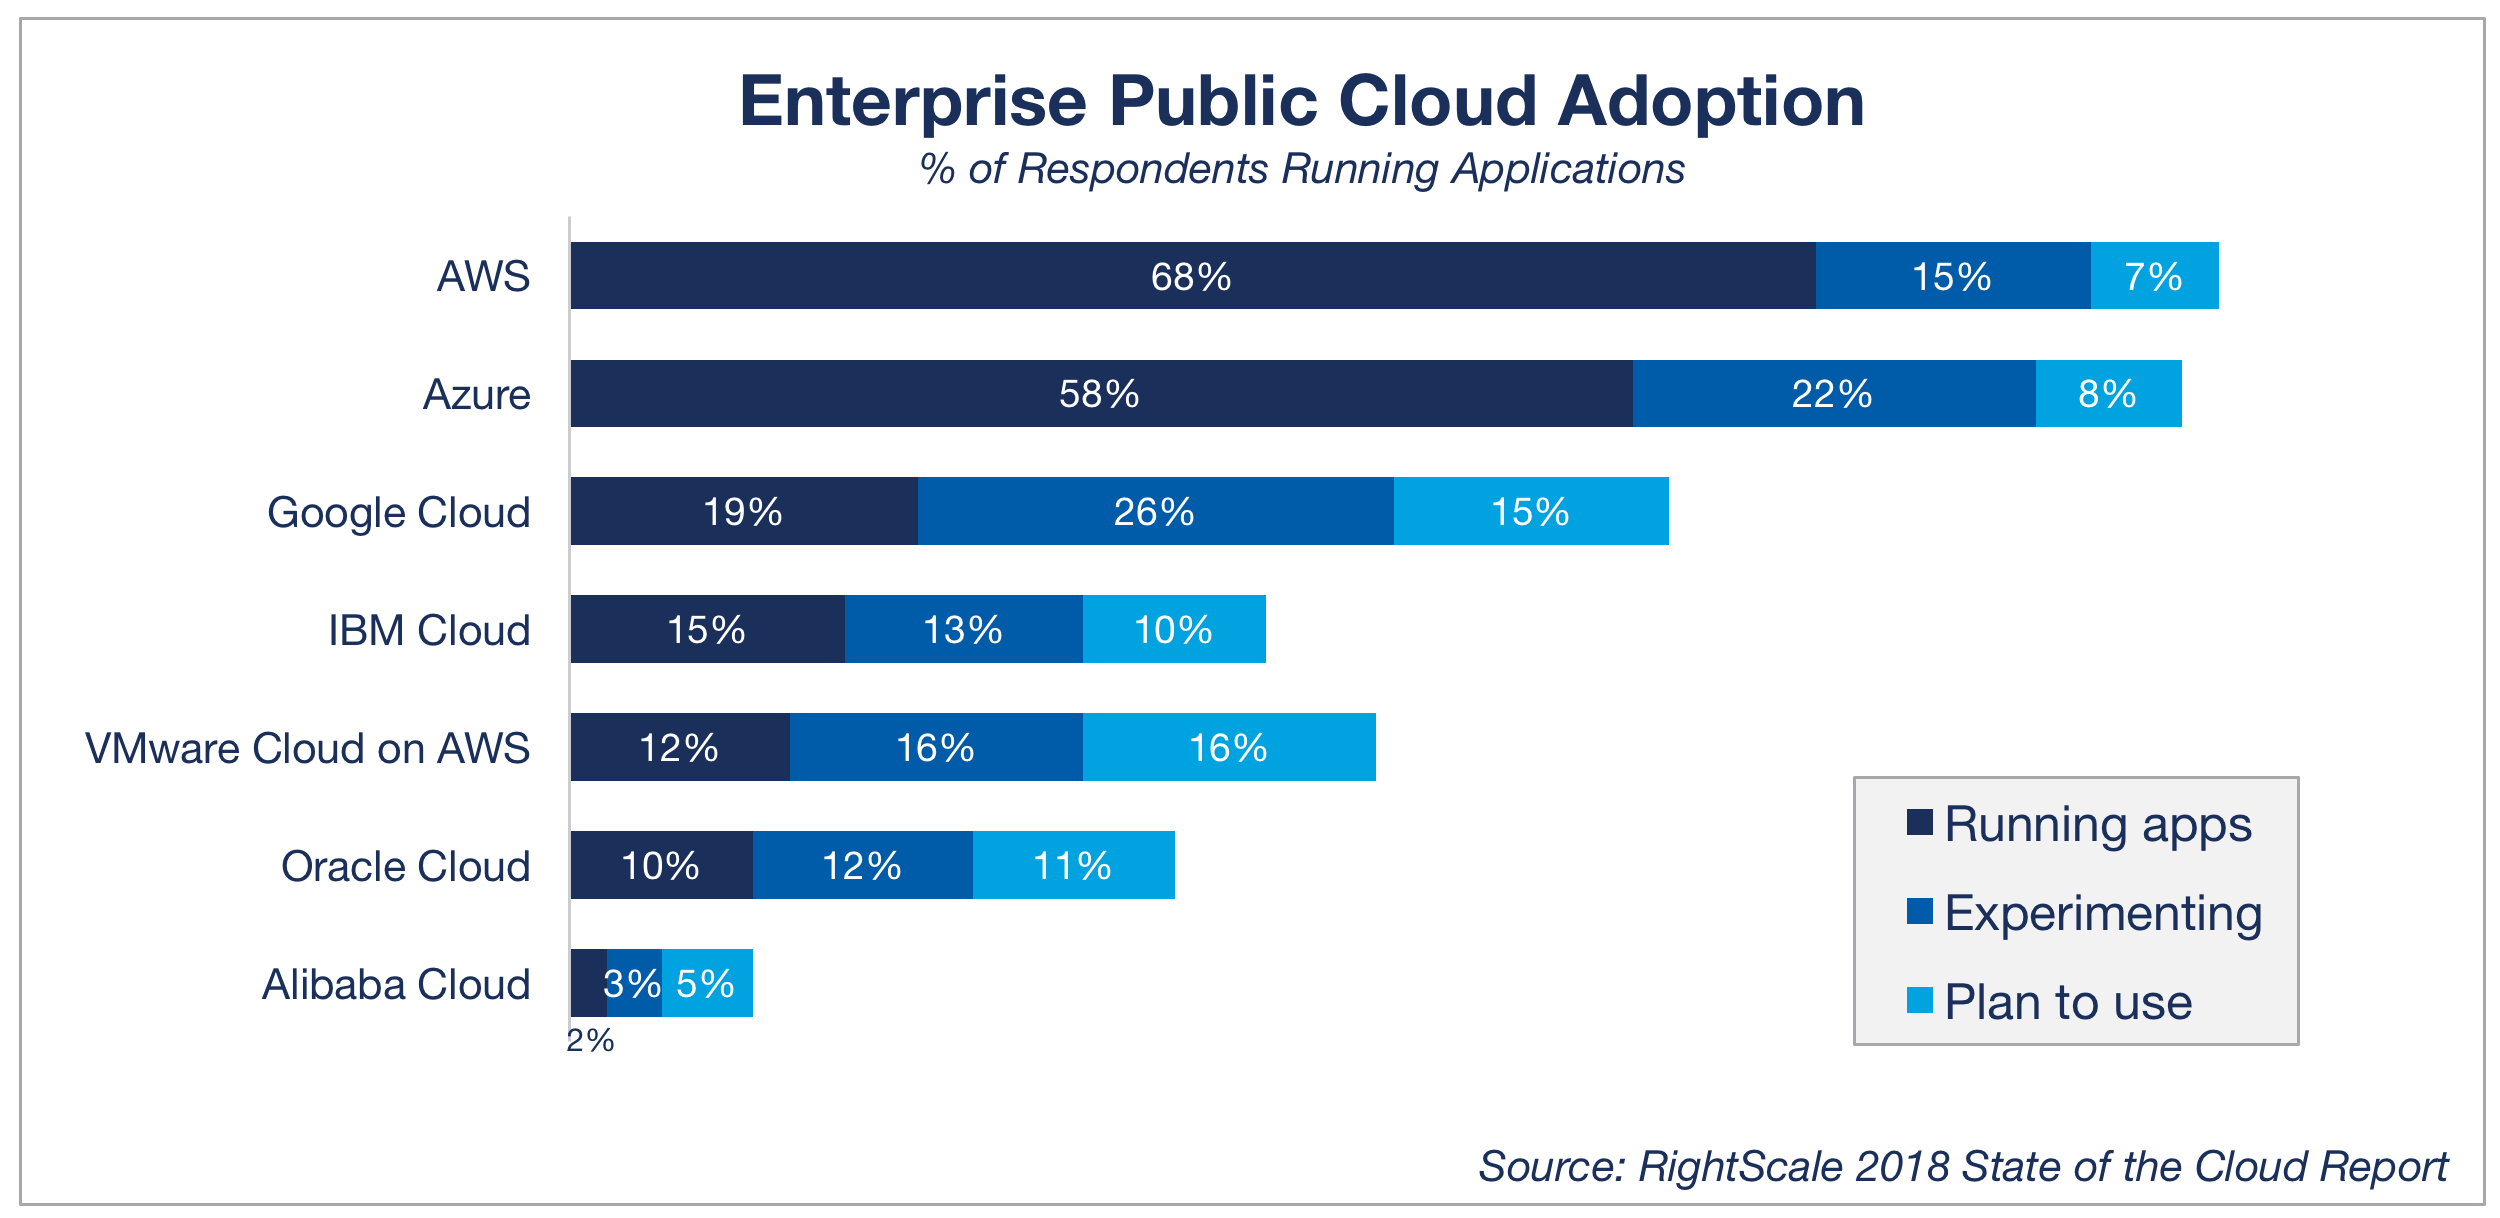
\includegraphics[width=1\textwidth]{23-Cloud-Computing-Trends-Enterprise-Public-Cloud-Adoption.png}
\caption{Felhőszolgátatónál a rendszerek minősítésének arányai, forrás: \cite{RightScale}}
\label{fig:CloudTrends2018}
\end{figure}

Jelneleg a többszáz szolgáltatás közül legdinamikusabban az adatbázisok és a serverless megoldások gyarapodtak, lásd \ref{fig:TopGrowingCloudServices}. Érthető, hiszen főleg az adatbázisoknál az adatmennyiség, és a feldolgozáshoz szükséges erőforrás közel exponenciálisan gyarapszik, így a hardverek ára közel csillagászati összegeket képes ölteni, főleg a mai üzleti helyzetben, amikor a memória chippekből hiány van. \\
\begin{figure}[H]
\centering
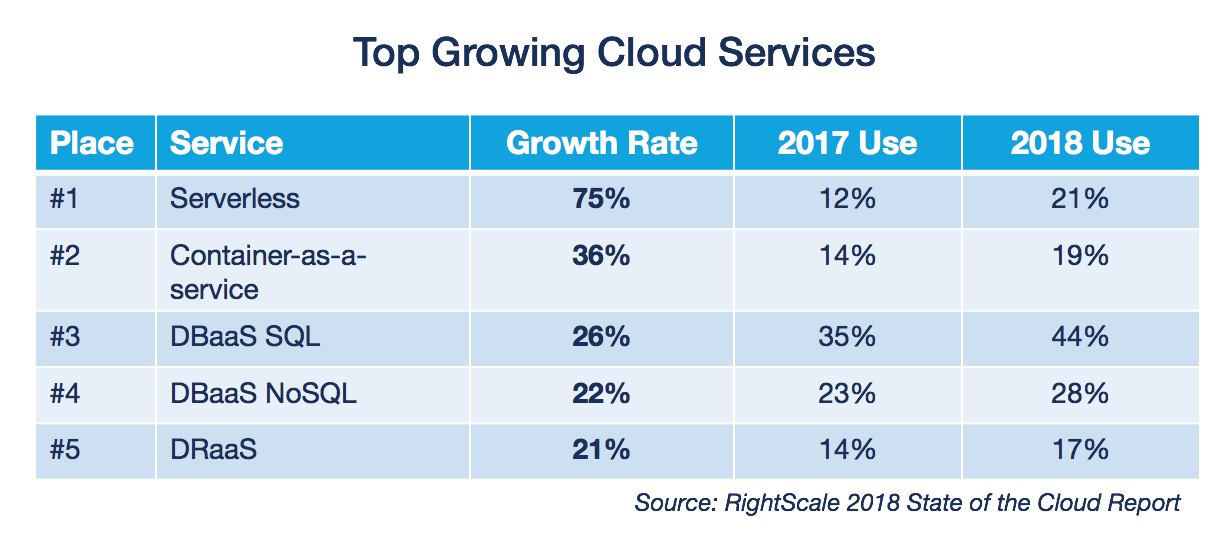
\includegraphics[width=1\textwidth]{6-Cloud-Computing-Trends-Serverless-Top-Growing-Cloud-Service.png}
\caption{Leggyorsabban növekedő felhőszolgáltatások, forrás: \cite{RightScale}}
\label{fig:TopGrowingCloudServices}
\end{figure}

\subsection{Microsoft Azure}
\begin{figure}[H]
\centering
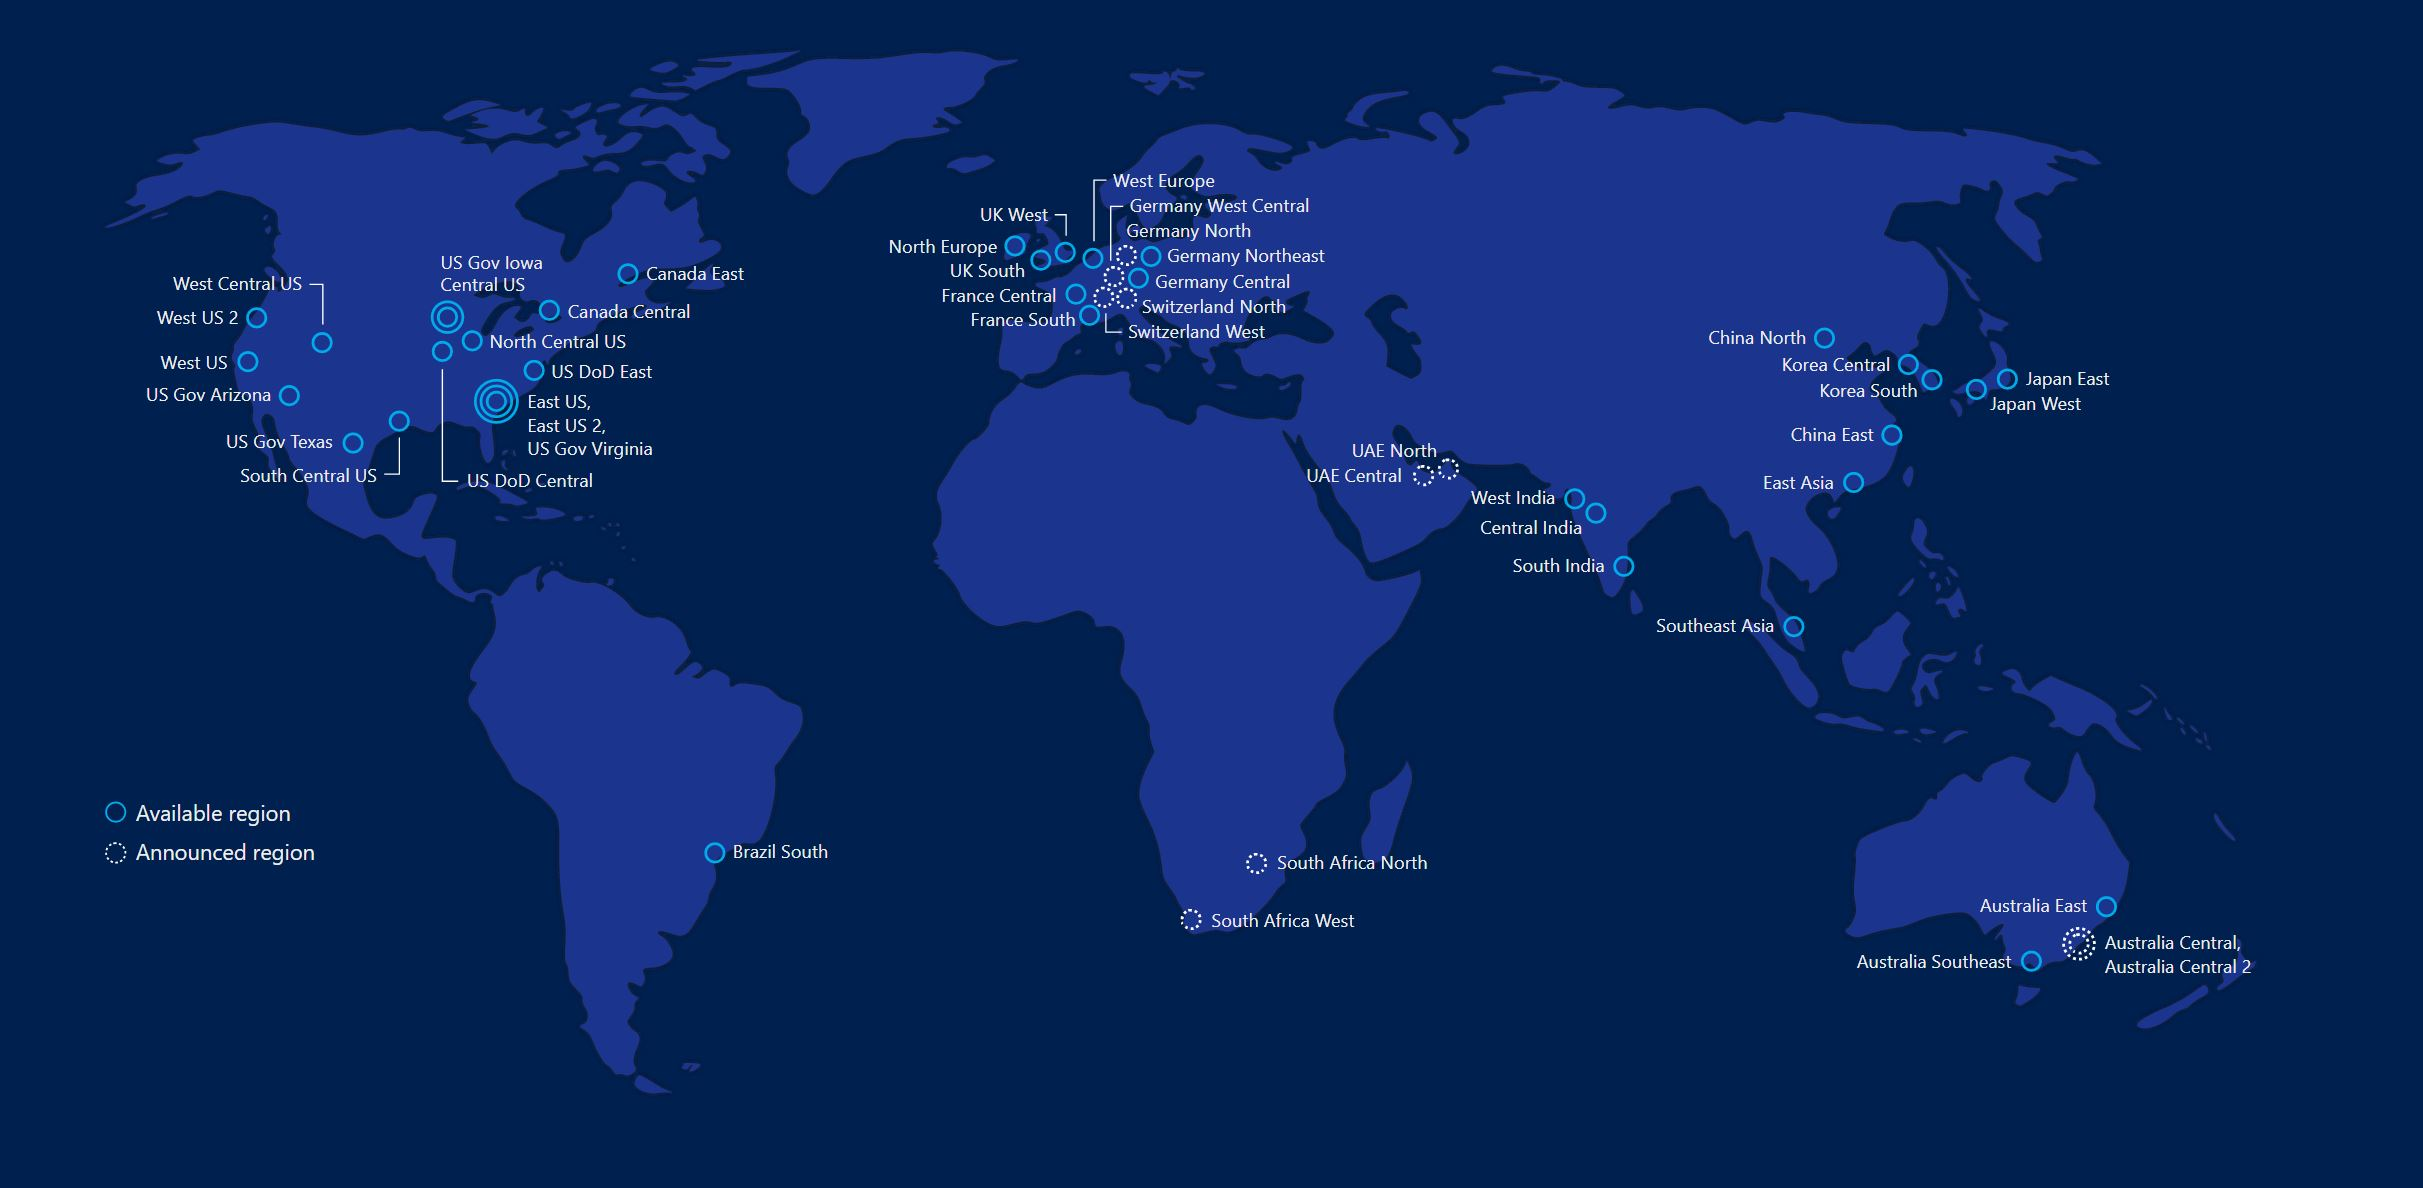
\includegraphics[width=1\textwidth]{azure_locations.jpg}
\caption{Azure adatközpont lokációk, forrás: \cite{Azure_Regions}}
\label{fig:AzureRegions}
\end{figure}
Eredetileg Windows Azure néven 2008 októberében jelentették be. Világszerte 50 régió, 140 országában találhatóak adatközpontjaik, ahogyan az a \ref{fig:AzureRegions} ábrán is látható. A kezdetektől fogva folyamatosan bővülő szolgáltatás kínálat jellemzi, így manapság már 600 szolgáltatás fölött kínálnak. A fontosabbak kategóriák: \cite{Azure_Services}\\

\noindent \textbf{Compute:}\\
Amennyiben felhős számítási kapacitásra, virtualizációra van szükség, az Azure on-demand szolgáltatásai a rendelkezésre állnak. A legkisebb osztott processzor időt kapó gépektől, egészen a fizikai hardverek felső korlátozásaiig, akár automatikus skálázással. Mint minden felhő szolgáltatás esetén itt is csak akkor és annyit kell fizetni amennyi felhasználásra került. \\

\noindent \textbf{Network:}\\
A felhőben futó rendszerek és a még on-premisses rendszerek között is meg kell teremteni az összesköttetést, hogy a felhasználók számára a legjobb élményt lehessen nyújtani. Legyen szó akár load balancer-ekről, site-to-site VPN-ről, DNS szolgáltatásról, DDoS védelemről, az Azure-ben mindezekre meglehet találni az alkalmas szolgáltatást.\\

\noindent \textbf{Storage:}\\
Skálázható felhőtárhely az adatok vagy a munkafolyamatok számára. Lényegében felső korlát nélkül lehet on-line tárhelyet rendelni az Azure szolgáltatásán keresztül, hiszen megfelelő konfiguráció esetén a tárhely mennyisége a tárolandó adatokkal együtt nő, így sosem akad meg a munkafolyamat azon, hogy nincs rendelekzésre álló tárterület. Archiválásra alkalmas tárhelyet is lehet vásárolni, amely nagyon alacsony költség mellett nyújt egy jó alternatívát, hiszen 0,002\$ / GB havonta amit a tárolásra kell fizetni, egyedül az adatok letöltésekor magasabb a költség 0,02\$. \\

\noindent \textbf{Database:}\\
Szinte mindegy milyen típusú adatbázisban vannak az adatok, vagy hogy milyen típusra van szükség az Azure-ben megtalálhatóak a legelterjedtebb adatbázismotorok. Amennyiben az adatbázis a Microsoft felhőszolgáltatásában került kialakításra az elérhetősége biztosan az SLA-ban meghatározott kereteken belül fog mozogni. A telljesítmény és a tárterület többet nem lesz gond, még akkor sem ha korábban alacsonyabb kategóriába tartozó rendszer lett igényelve. \\

\noindent \textbf{Security + Identity:}\\
Amennyiben a rendszereket függetleníteni kell az előre megvásárolandó hardverektől és rendszerektől. Telljes Active Directory struktúrát lehet a felhőben építeni, amely biztosan mindig elérhető lesz, amennyiben a kapcsolatot a felhővel fel tudja építeni a kliens. Napjainkban a többlépcsős azonosítás már kötelező tényező az adat és személyiség védelemben. Az Azure-ből egy kész megoldást lehet ilyen célra is bérelni. \\

\noindent \textbf{Developer Tools:}\\
Komoly feladatot jelent minden fejlesztést végző cég adminisztrátorai számára a megfelelő platform megtalálása, megépítése, üzemeltetése. Elvégre a fejlesztők napi munkálya múlik azon, hogy elérik-e a kódokat amelyeken dolgozniuk kell. A Microsoftnak természetesen erre is van megoldása, támogatja a legfőbb platformokat, igény esetén konzultációs szolgálatatásokat is igénybe lehet venni. \\

\noindent \textbf{Management Tools:}\\
Az üzemeltetés minden rendszernek a leghosszabb életciklusa. Ugyan telljesen autonóm módon nem képes a rendszer működni, de egy hagyományos on-premises infrastruktúrához képest jelentősen kisebb személyzet is képes egy telljes céget kiszolgáló infrastruktúrát üzemeltetni. A mindennapi munka megkönnyítésére létezik az Automation amely egy Orcestrator, így a támogatott rendszerk közül bármilyen technológia beköthető, legyen az a felhőben vagy lokálisan az adatközpontban. A Traffic Manager több mint egy szimpla terhelés elosztó, lokáció alapon képes mindig a legközelebbi (legkisebb késleltetésű) végponthoz irányítani a kommunikációt. 

\subsection{AWS Cloud}
Az első cloud szolgáltatás 2006-ban vált elérhetővé a nagyközösség számára. Ebben az évben még csak tárhelyet és számítási kapacitást lehetett elérni. Napjainkban 54 zónát számlálnak 18 geográfiai régión keresztül, ezek a számok folyamatosan bűvülnek.
\begin{figure}[h]
\centering
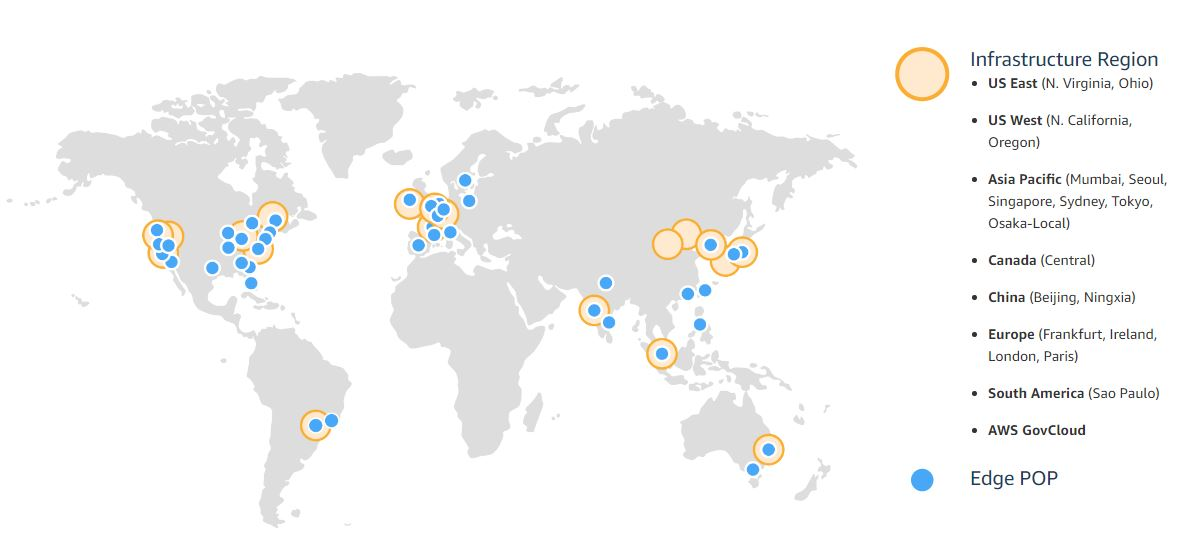
\includegraphics[width=1\textwidth]{aws_locations.jpg}
\caption{AWS adatközpont lokációk, forrás: \cite{AWS_Regions}}
\label{fig:AWSRegions}
\end{figure}

Természetesen az Amazon mint a legnagyobb cloud platform szolgáltató, szolgáltatások széles választékát nyújtja. Az elsőségét komolyan fenyegeti a Microsoft megoldása, rohamosan jönnek fel az évek során, amint az a \ref{fig:CloudAdoption2017-2018} ábrán is láthattuk.  \\

Jelenleg még jól látható, hogy a cégek kisebb lábnyommal rendelkeznek a felhőben, lásd \ref{fig:VMsPerCompany}. Nagyon alacsony azok száma akiknek többszáz virtuális gépe futna. 
\begin{figure}[H]
\centering
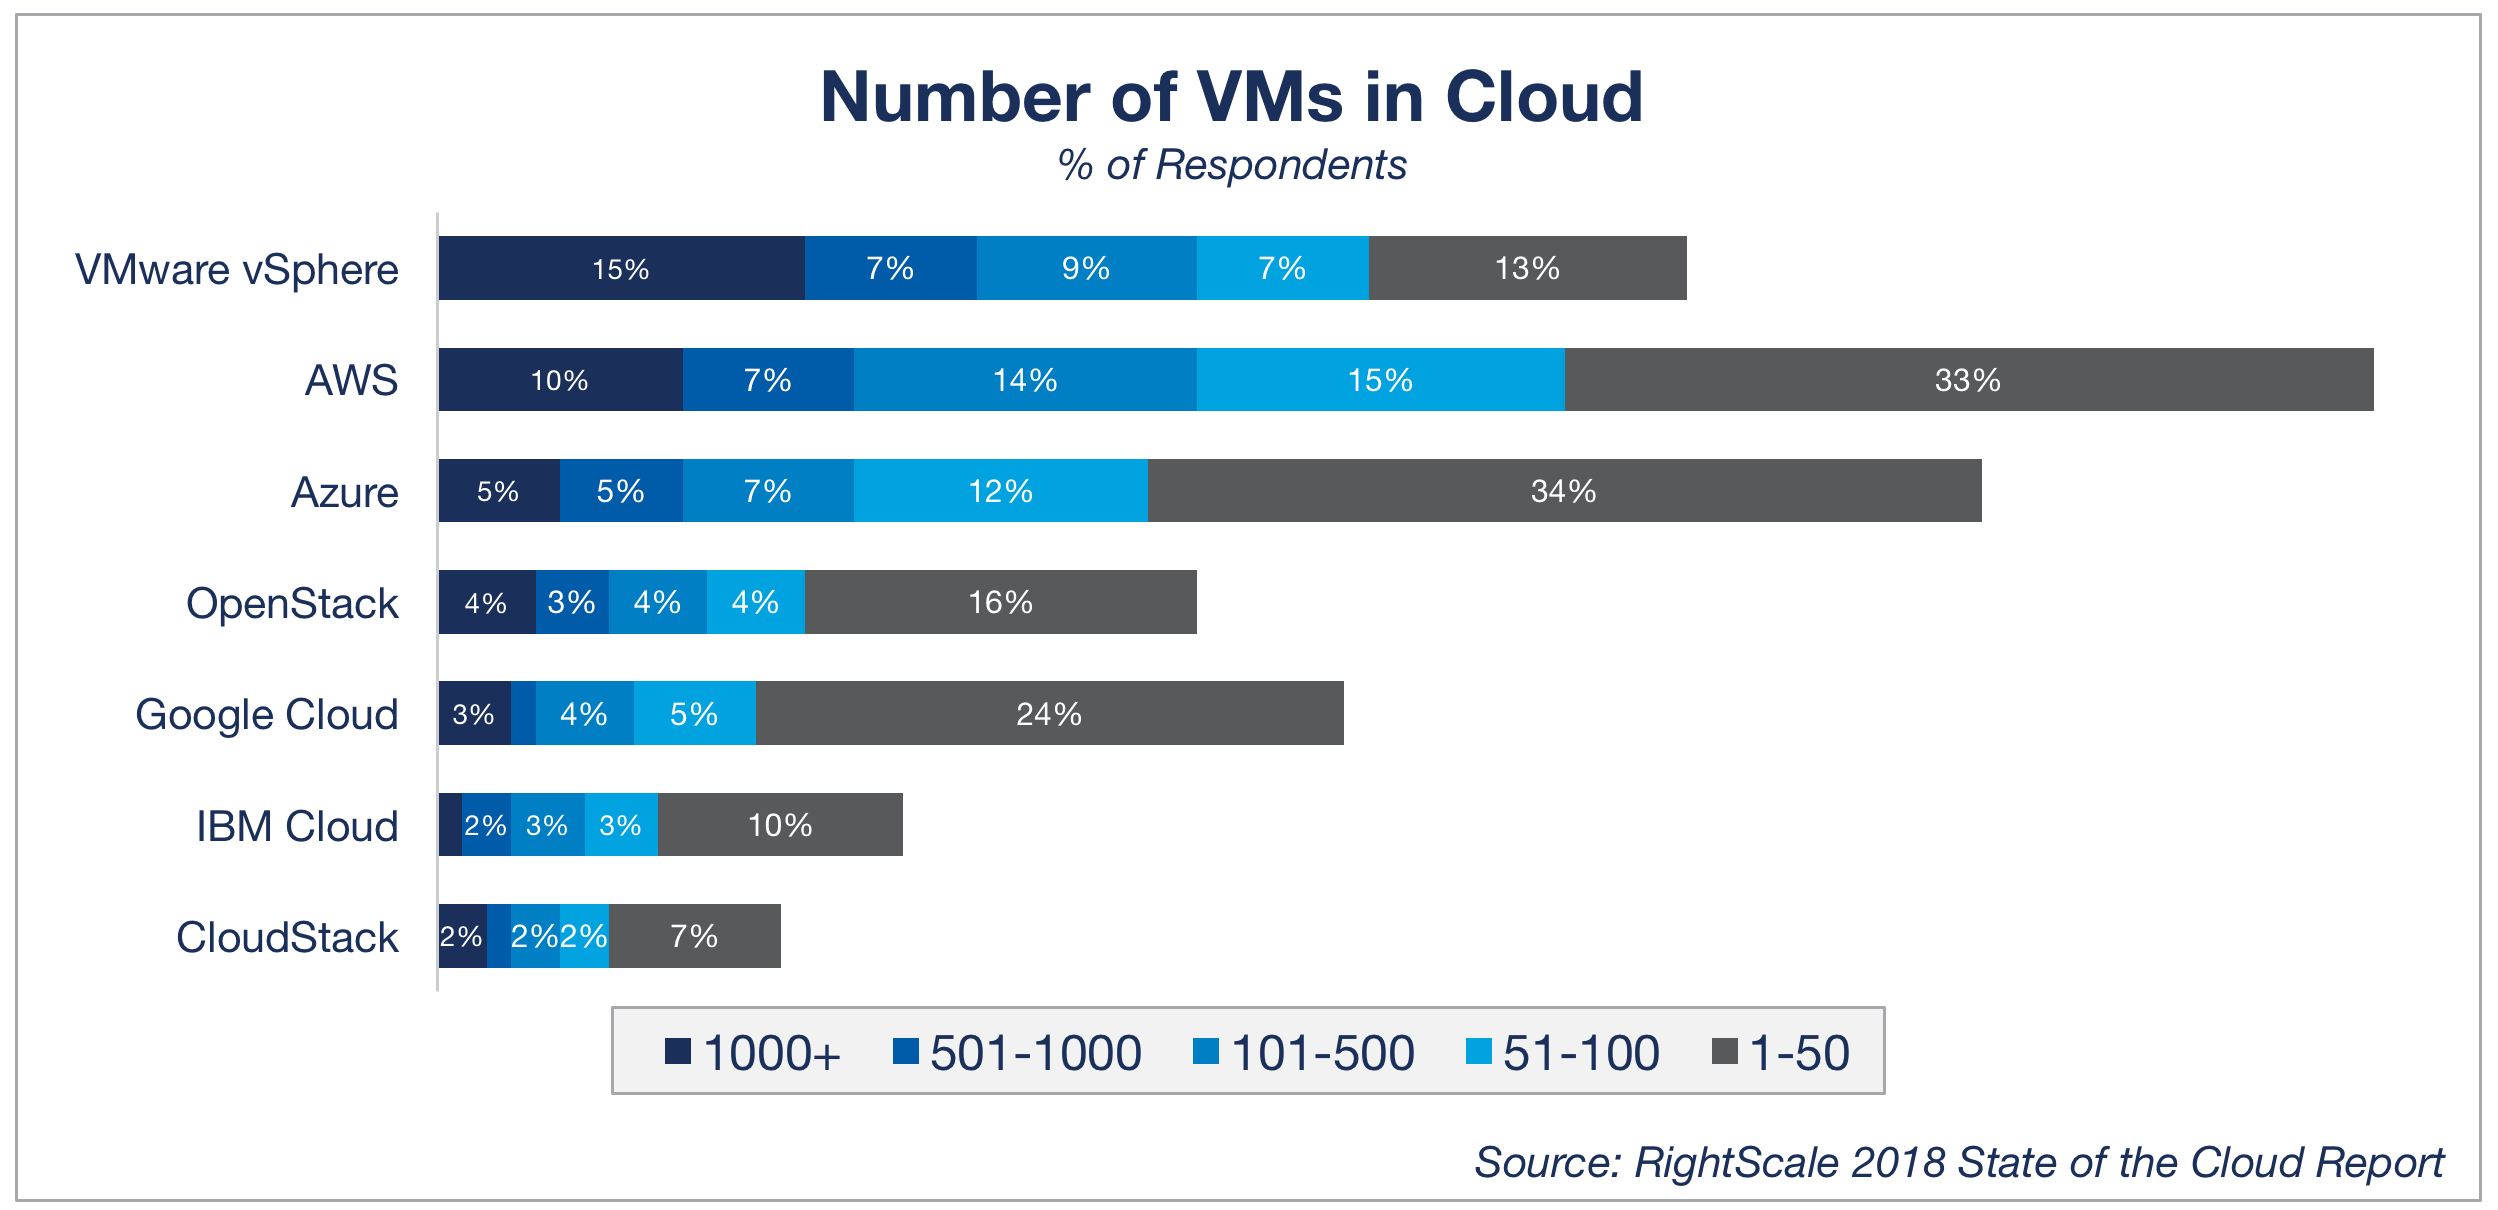
\includegraphics[width=1\textwidth]{26-Cloud-Computing-Trends-Number-of-VMs.png}
\caption{Virtuális gépek számának eloszlása cégenként, forrás: \cite{RightScale}}
\label{fig:VMsPerCompany}
\end{figure}

\chapter{Esettanulmány}

A diplomamunkám megírásakor nem állt rendelkezésre, olyan alany akinek az esetét fel lehetett volna dolgozni, így egy feltételezett igénylőt alkottam meg és azt vezetem végig. \\

Az inspirációmat a manapság igen divatos Start-Up cégekből merítettem. A startupok olyan vállalkozások amelyeket frissen alapítottak, gyorsan növekednek, céluk pedig valamilyen piaci igény kielégítése. Ezen cégek általában közepes méretű vállalkozások, amelyeknek az üzleti modelljének legfontosabb építőköve a nagymértékű növekedés. Többségében a manapság igen dinamikusan változó területeken ténykednek, például: internetes szolgáltatások, informatika, távkommunikáció és robotika. Azért tudnak ilyen hatékonyak lenni, mert a tervezésben, fejlesztésben, tesztelésben és a kutatásban is részt vesznek. Mivel nem csak informatika területén mozognak a startup-ok, így az elnevezés a 1990-es években elterjedt a hasonló üzleti modellt követő vállalkozásokra is.
Amint azt már fentebb leírtam, ezeknek a vállalkozásoknak ingadozó a növekedési ütemük, ezzel együtt az erőforrás igényük nehezen tervezhető.  Az állandóan változó igényeket sokkal könyebb kielégíteni ha IaaS modellben dolgoznak.\\

\noindent \textbf{IaaS} - Infractructure as a Service \cite{IaaS}

Átmenetet képez a klasszikus infrastruktúrális kiépítés és a teljesen felhőből kiszolgált rendszerek között. A szolgáltató ilyen esetben nyújta a biztonságos és stabil szolgáltatássokkal ellátott adatközpontot és a szervert, továbbá vállalja a fizikai üzemeltetést, lásd: \ref{fig:aaS} ábra. Mindent ami erre épül (operációs rendszer, alkalmazások, adatok) az igénylő üzemelteti és kezeli. 
\begin{figure}[h]
\centering
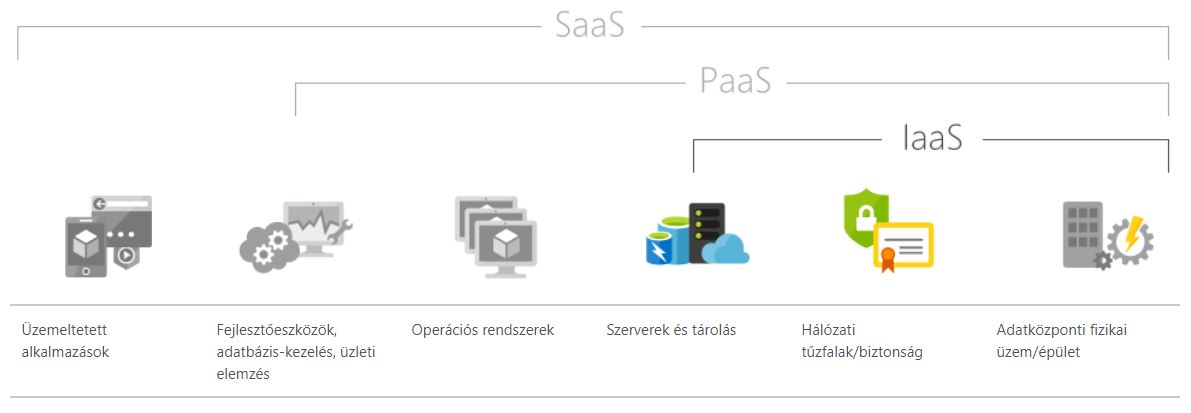
\includegraphics[width=0.9\textwidth]{aaS.jpg}
\caption{Szolgáltatási szintek}
\label{fig:aaS}
\end{figure}

\section{Igényfelmérés}
Minden esetben nagyon fontos az igényfelmérés. Egyrészről szükséges ahhoz, hogy a megrendelő a végén úgy érezze, hogy mindent megkapott amit szerett volna. Másrészről a szolgáltatót is fedezi, mert egy korábban megállapított és közösen elfogadott követelmény rendszernek megfelelő terméket ad át. Üzemeltetésnél elsőre nem tűnhet annyira fontosnak, mint fejlesztésnél, ellenben itt a legfontosabb előre kikötni, hogy mit is tartalmaz a támogatás, mennyi a normálisnak tekinthető rendelkezésre állási idő. Ezeket az Service Level Aggreement - továbbiakban SLA - dokumentumban kötik ki a felek. \\
Az igényfelmérés több lépcsőből áll. 
\subsubsection{Elbeszélgetés}
Ez az első lépése a követelmények felmérésének. Ez a szekció egyszer történik meg, ilyenkor a megrendelő és a szolgáltató egy embere - akik nem feltétlenül rendelkeznek technikai tudással - egy megbeszélés során összeszedik, hogy mit szeretnének elérni. 

\subsubsection{Technikai feltételek meghatározása}
Ez a feltárási művelet akár többször is megtörténhet még mielőtt elérnék a végső állapotot. Ebben a szekcióban már a technikai megbeszéléseknek is meg kell történni. 
Meg kell határozni a következő tényezőket:
\begin{itemize}
	\item Operációs rendszer meghatározása - ha lényeges a keretrendszer miatt
	\item A keretrendszer kiválasztása
	\item A hardver specifikációnak méretezése - fejlesztés, teszt és élő rendszerekre
	\item A front-end és back-end rendszerek meghatározása
	\item Egyéb kapcsolódó szolgáltatások feltárása 
\end{itemize}


\section{Ajánlat}

% TODO

%\section{Migráció cloudba}

\chapter{Esettanulmány háttércég}

\section{Architektúra}

Architektúrális szempontból Intel alapú szervereket használtam. A fejlesztői és tesztelői környezet alapját 2 db Dell PowerEdge R710-es szerver adta. A szerverek a munka ideje alatt egyenként 2 db Intel Xeon E6545 processzorral (6 mag 12 HT szál), 96 GB DDR3 ECC RAM-al, 2x64 GB rendszer lemezekkel illetve 2x136 GB adatlemezzel volt ellátva. A kettő szerver egy failover cluster-ben üzemelt. A rendszer és az adat lemezek RAID1-ben üzemeltek az adatvesztés megelőzése és a magas rendelkezésre állás biztosítása érdekében. Az adatlemezek mérete sosem volt gond a Windows Deduplikációs megoldása miatt.

A rendszereket központilag nem menedzselt, de egységes alapkonfigurációval láttam el annak érdekében, ha az ügyfélnek segítségre lenne szüksége. \\

\noindent A megépített rendszerben használt alapkonfiguráció:
\begin{itemize}
	\item Processzor: 2 mag
	\item Memória: dinamikus memória 1 GB minimum, 2 GB induláskor, 4 GB maximum.
	\item Háttértár: 64 GB Operációs rendszer lemez, 32 GB Adat lemez
	\item Hálózati kártya: 1 DB a megrendelő rendszerinek a belső hálózatán
	\item Operációs rendszer: Windows Server 2012 R2
\end{itemize}

\subsubsection{Lite touch deployment}
Fontos szempont, hogy egy megrendelt rendszer mennyi időn belül lesz használatba vehető és a megrendelések előkészítése mennyi időt vesz igénybe a szolgáltató cég részéről. Alapvetően 3 irányzatot lehet felismerni a rendszerek elkészítését illetően.\\

Ha a klasszikus IaaS szemléletet vesszük alapul, akkor a szolgáltatónak csak a szervert vagy a virtuális gépet kell előkészíteni, hozzáférést garantálni és a rendszer használatba is vehető. Az elkészítésre fordított szinte minimális hiszen virtualizált rendszerek esetén akár teljesen automatikusan is megtörténhet minden lépés a megrendeléstől az átadásig. Amennyiben fizikai hardvert használ a megrendelő, akkor elő kell készíteni a hardvert az adatközpontban és a megfelelő konfiguráció elkészítése után adható csak át. Természetesen ilyenkor az operációs rendszer telepítése a végfelhasználóra marad. \\

A következő lépcsőfok, amikor az operációs rendszert és alkalmazásokat is előtelepítve adjuk át a rendszereket. Fontos megemlíteni, hogy nem minden megrendelést lehet valamilyen előre megalkotott rendszerrel kiszolgálni. Ugyanakkor az esetek jelentős részét előre definiált alkalmazás palettával le lehet fedni. A Microsoft létrehozott egy Lite Touch megoldást amelyet Microsoft Deployment Toolkit-nek nevezett - továbbiakban MDT. Az MDT nagy előnye hogy az operációs rendszer feltelepítését, annak konfigurálását és az olyan alkalmazások telepítését amelyek rendelkeznek felügyeletlen telepítővel teljesen automatikusan elvégzi. Amennyiben olyan módosítást szeretnénk elvégezni, amely nem automatizálható, úgy a telepítés addig felhasználói beavatkozásra vár. Azért hívják lite touch-nak mert ténylegesen csak azoknál a lépéseknél igényel felhasználói interakciót amelyeket nem tud magától elvégezni és a telepítés elindításkor. Az MDT univerzális eszköz mert alkalmas virtuális gépek és fizikai hardverek telepítésésre is, ugyanakkor a fizikai gépek esetén még a driverek telepítését is elvégzi. Az MDT előnye egyben az egyik hátránya is. A teljes telepítéshez szükséges adatmennyiséget át kell vinni a hálózaton és a telepítéskor jelentkező terhelést a hardverre nem lehet lecsökkenteni. Alapját a Preboot eXecution Environment - továbbiakban PXE - adja amely egy nagyon kisméretű rendszer, ez hozzáférést garantál a hardverhez és elvégzi az operációs rendszer telepítés részeit, a többi beállítást már a windows telepítés post-install szekciójában maga a rendszer futtatja le.  \\
\begin{figure}[h]
\centering
\includegraphics[width=1\textwidth]{mdt.png}
\caption{MDT telepítési képernyő, forrás \cite{MDTImage}}
\label{fig:mdt_image}
\end{figure}

Hasonló megoldás, de másabb megközelítés amikor egy admin előtelepíti a rendszert, feltelepít és beállít minden olyan alkalmazást amire szükség van abban a rendszerképben, amint végzett úgy a rendszeren végrehajt egy preparálást. A preparálás után a rendszerkép bármilyen kompatibilis hardverrel rendelkező gépre alkalmazható. Amennyiben ezt a technológiát használják az adminisztrátorok, megspórolhatják a bonyulult és nem automatizálható alkalmazások telepítését minden egyes új rendszer üzembe helyezésekor. Amikor virtualizált környezetből szolgálják ki az igényeket, előnyös lehet ezt használni, ugyanis a hardver biztosan kompatibilis lesz. Az MDT-vel ellentétben itt csak az elkészült lemezképet kell átvinni a hálózaton, aztán csak el kell indítani és használatba is vehető, a telepítés hardverterhelése csak a mester lemezkép elkészítésekor jelentkezik. \\

Az előbb látott módszereket tovább lehet fejleszteni, ellenben az már külön alkalmazáscsomag megvásárlását igényli. A Microsoft System Center alkalmazáscsomag része a Configuration Manager. Amennyiben rendelkezik a szolgáltató ezzel az alkalmazással, úgy elérhető bizonyos esetekben a Zero Touch telepítés is. Megjegyzendő, hogy a Zero Touch csak akkor fogható fel ténylegesen nulla interakciót igénylő telepítésnek, ha egy UEFI-re alkalmas már telepített operációs rendszerrel és SCCM agent-el rendelkező gépet kell újratelepíteni. Ezen kritériumok fennállása esetén az SCCM agent képes úgy újraindítani a gépet, hogy nem kell még a PXE boot menüt sem manuálisan felhozni, ahonnan automatikusan a megfelelő konfigurációs lemezképet fogja a telepítő betölteni. 

A dolgozat elkészítésekor én preparált rendszerképeket használtam. Számomra ez volt a legelőnyösebb, mert a cluster közös tárolóhelyén volt letárolva a mester lemezkép. Egy új rendszer létrehozása másodpercekben mérhető, mert a deduplikációnak köszönhetően nem kell a rendszernek mozgatni 30GB-nyi adatot, csak létrehozza az újraelemzési pontokat.  

\subsubsection{Dashboard}
\begin{figure}
\centering
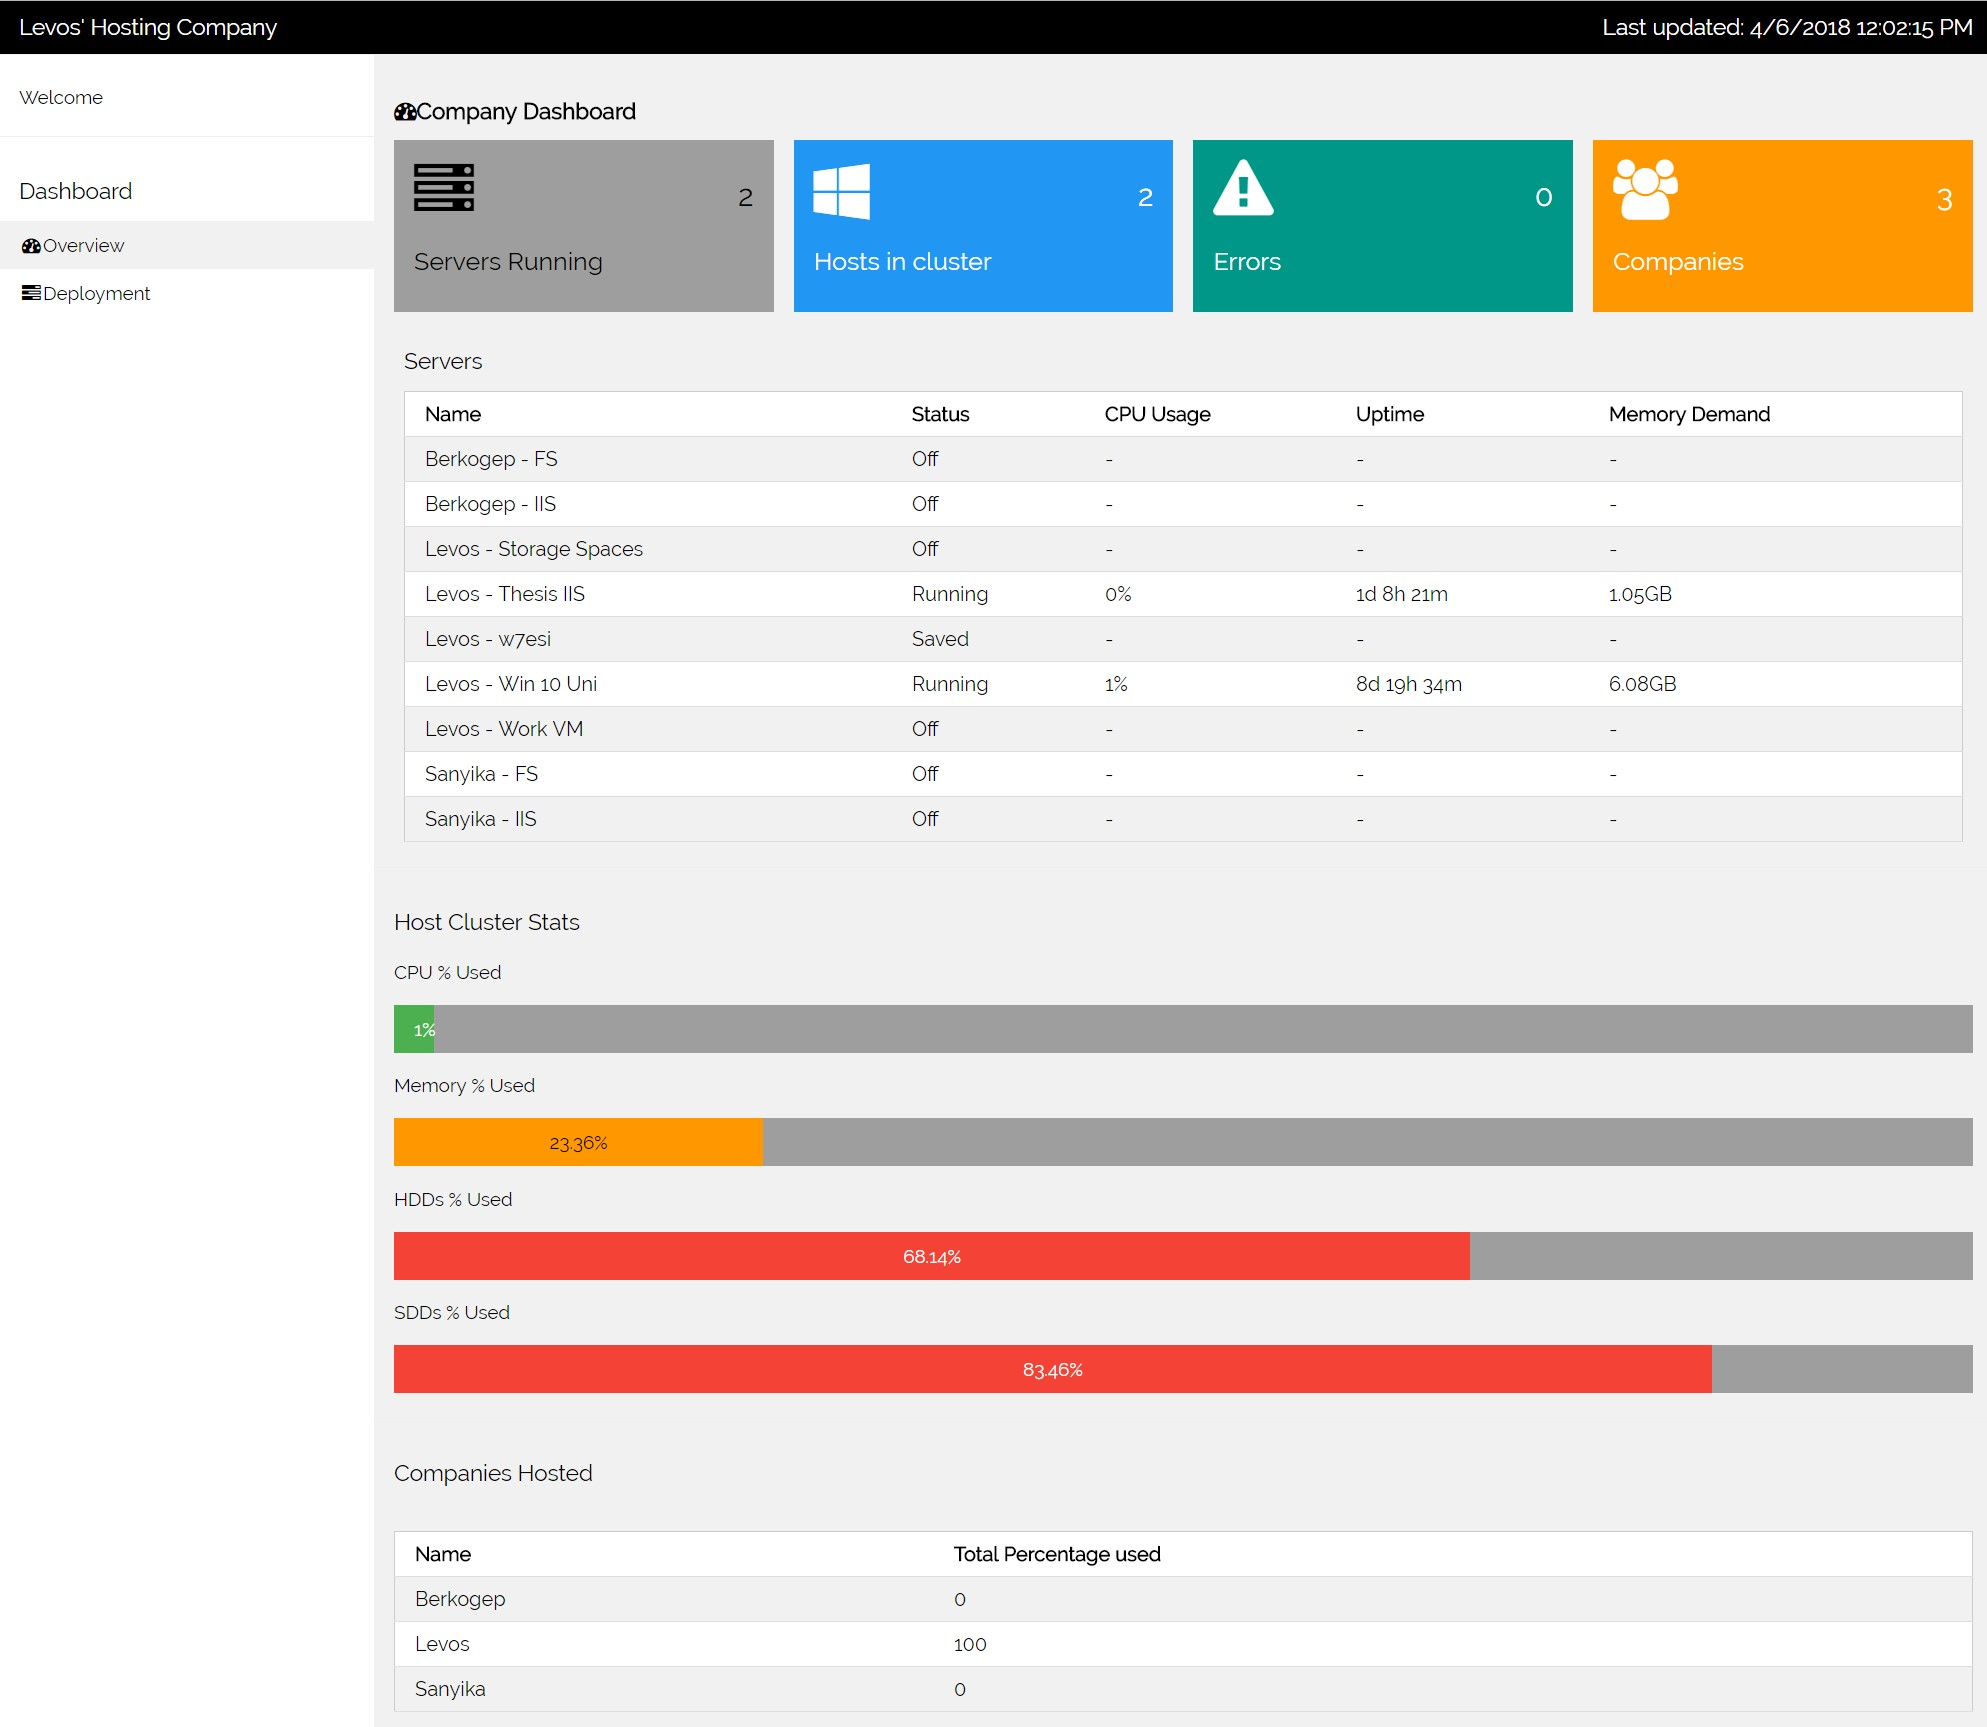
\includegraphics[width=1\textwidth]{dashboard.jpg}
\caption{Az áttekintő nézetben minden szükséges és fontos információ megtekinthető}
\label{fig:owndash}
\end{figure}

\begin{figure}
\centering
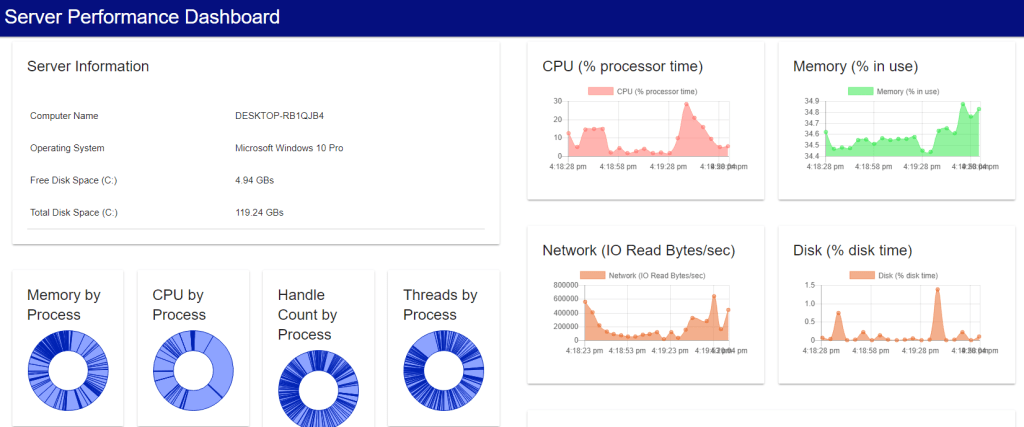
\includegraphics[width=1\textwidth]{psudashboard.png}
\caption{PowerShell Universal Dashboard példa, forrás \cite{poshtools}}
\label{fig:psudash}
\end{figure}
Az üzemeltetést végzők számára előnyös, ha van egy olyan felület amelyen minden lényeges információt látni lehet. Létezik tisztán PowerShell alapú megoldás dashboard készítésre, de a PowerShell Unviersal Dashboard az én esetben nem tökéletes megoldás \cite{poshtools}. Fontos limitáció, hogy a működéséhez szükség van egy olyan szerverre amelyről minden erőforrás elérhető és azokon képes PowerShell parancsokat futtatni, továbbá licence köteles termék. Az én rendszerem úgy van megépítve, hogy nem igényel semmilyen plusz beruházást az operációs rendszeren és a hardver árán felül. Ezek mellett a saját implementációm úgy van felépítve, hogy egyetlen rendszernek kell hozzáférnie egy közös tárolóhelyhez. A közös tárolóhelyen találhatóak a gazdagépek statisztikáját tartalmazó fileok, illetve a webfelületen keresztül leadott kérelmek adatai. Az rendszer amely eléri ezeket a fileokat frissíteni tudja a dashboard-ot az adatoknak megfelelően - lásd \ref{fig:owndash}.

\subsubsection{Deployment}
A weboldal további funkciója közétartozik a rendszerigénylési űrlap. Ezen az oldalon az igénylő leadja a kérelmét a megfelelő adatok megadásával. Ebből aztán készül egy kérés, amelyet később egy ütemztett feladat feldolgoz és végrehajt. Lényeges mező a karbantartási időablak. Ezt az igénylő a kérlem leadásakor ad meg, de van módja későbbiekben is módosíttatni. Ez az időablak egy a felhasználóval kialkudott közös sáv, amikor a rendszer autmatikusan elvégezheti az olyan módosításokat amelyek leállással vagy újraindulással járnak. Ilyen módosítás például a processzor magok számának módosítása, vagy egy új hardver hozzáadása, természetesen a frissítések telepítése utáni újraindítás is megtörténik ebben az időszakban. A rendszer ad lehetőséget arra, amelyet a konzultáció során külön lehet kérvényezni, hogy bizonyos alkalmazást kiszolgáló szerverek ne legyen egy karbantartási idősávban, így növelhető a rendelkezésre állás. 

\section{Automatizált megoldások}

\subsection{On-Premisess}


Az automatizált rendszer első és legfontosabb építőköve a virtuális gépek gyors elkészítése. Mivel az esettanulmányban egy szolgáltató céget tételeztem fel, így fontos volt, hogy minél kevesebb interakcióval, lehetőleg teljesen automatikusan lehessen legyártani az igényelt virtuális gépeket. A virtulális gépek legyártása és menedzselése megoldható egy webfelületről.

\subsubsection{Provision-ObjectsForCompany.ps1}
Egy gyűjtő kód amely megfelelően paraméterezve elvégzi a teljes virtális gép létrehozás lépéseit. 
A következőkben taglalt scripteket hívja meg. 
A kódok végrehajtása az előkövetelményeknek megfelelően történik:
\begin{enumerate}
	\item Virtuális Switch létrehozása (Crete-NewVirtualSwitch.ps1)
	\item Viruális gép(ek) létrehozása (Create-VM.ps1)
	\item A virtális gépek hálózatba fűzése (Set-VMSwitchForVM.ps1)
\end{enumerate}

% \\TODO

\subsubsection{Create-NewVirtualSwitch.ps1}

Virtuális switchek tulajdonságát korábban taglaltam. A cégnél a megrendelők rendszerei teljesen elszeparált rendszerek, hacsak a megrendelők másképp nem rendelkeznek. Ellenben a virtuális gépek amelyek egy megrendelőhöz kötődnek egymással közös hálózaton vannak. Szolgáltatói oldalon a cégekhez tartozó erőforrások azonosítása érdekében a megrendelő cég nevét eléfűzöm az erőforrás nevéhez. Amennyiben már létezik ilyen erőforrás úgy a script küld egy email üzenetet az üzemeltetőnek, hogy manuális ellenőrzésre van szükség.

\subsubsection{Create-VM.ps1}

A script egy az argumentumaiban szereplő paramétereknek megfelelő VM konténert hoz létre. A beállításokat tekintve, ha valamelyik paraméter nincs felülbírálva az argumentumokban, akkor a korábban már taglalt alapbeállítás kerül felhasználásra.

A script úgy lett elkészítve, hogy képes felismerni ha valamelyik lemez VHDX állománya már létezik.
% \\TODO

\subsubsection{Post-Configuration.ps1}
% \\TODO

\subsubsection{Update-WebPage.ps1}
Mint azt már korábban említettem a rendszer működését egy weboldalon keresztül nyomon lehet követni. A webfelületnek van egy általános áttekintő nézete, amely a rendszeradminisztrátor számára ad egy képet pillanatnyi állásról. 
Biztonsági szempontokból a a weblapot frissítő kódot nem olvashatja a cluster adatait, így a hostokról a webfelület számára fontos információkat a Get-HostStatistics.ps1 script gyűjti össze majd menti le egy olyan helyre amelyre van olvasási joga a jelenlegi scriptnek. Ezt az adatállományt dolgozza fel és vizualizálja. A webfelületen megjelenik az összes VM fontos tulajdonsága, a cluster kihasználtságára vonatkozó adatok, illetve a hostolt igénylők egymáshoz viszonyított erőforrásigénye.

A HTML kódot a Powershell XML modulján keresztül szerkesztem, a szükséges számításokat a frissítéskor számítja ki a script.

\subsubsection{Get-HostStatistics.ps1}
Biztonsági szempontból a weboldalt aktualizáló kódnak nincs még olvasási hozzáférése sem a cluster-hez. Ez a megoldás egyébként garantálja azt is, hogy mindegy hol van a világban a host vagy cluster, ha a közös tárterületre képes az adatait lementeni, beolvasztható a jelenlegi rendszerbe. 

Üzemeltetés szempontjából lényeges, hogy az adott gazdagépek processzora és memória készlete mennyire van kihasználva, ám még fontosabb információ a rendelkezésre álló tárterület. Éppen ezeket az információkat kérdezi le a script és tárolja le. Az adatokat -  Powershell objektumok - exportálom XML fáljba, így megőrzök minden információt amelyet később vissza lehet nyerni a feldolgozás során.

\subsection{Cloud}
\noindent


\chapter{PowerShell}
A shell mint fogalom az informatikában a kezdetektől fogva létezik. A shell tulajdonképpen nem más, mint egy interfész amely lehetővé teszi a felhasználó és az operációs rendszer közötti interakciót. A shell lényegében nem egy alkalmazás a megkerülhetetlensége miatt, de nagyon hasonló bármely más folyamathoz a rendszerben. A shell-ek attól függően, hogy milyen operációs rendszeren találhatóak, lehetnek parancssoros (UNIX, Linux, VMS) vagy grafikus interfészek (Windows vagy Mac OS X). Továbbiakban az angol terminológiából származtatott rövidítéseket fogom használni, a parancssoros felületre a Command-Line Interface azaz CLI-t, míg a grafikus interfészre a Graphical User Interface azaz GUI-t.

Mind a két shell-nek megvan az előnye és a hátránya. Az átlag felhasználó számára a GUI előnyösebb, mert nem igényel annyi előzetes tudást az adott rendszerrel kapcsolatban, elég ha a GUI-k általános használatát ismeri. Ebből kifolyólag a fejlesztésükkor nem volt szempont, hogy az egyik parancs kimenetét egy másik fel tudja dolgozni. 

A CLI-nek megvan az a nagy előnye, hogy a parancsok kimeneteit egy másik parancs fel tudja dolgozni, ugyanakkor mivel parancssoros felülete van a felhasználónak mélyebb tudással kell rendelkeznie a használatához.

Habár léteznek GUI shell-ek, a shell-t mint fogalmat valamilyen CLI-re használják. Ugyanis a shell programozás is azt a cselekményt takarja amikor a megfelelő parancsok sokaságát összegyűjtjük amit egyébként a CLI-be táplálnánk vagy futtatható állományként átadnánk.
\cite{WindowsPowerShellUnleashed}

\subsubsection{A shell-ek története}
Az elsőkörben elterjedten használt shell a Bourne shell volt, amely a UNIX rendszerek alapértelmezett felhasználói felülete is egyben. C fejlesztőknek készítették C fejlesztők, ám mégsem C-szerű szintaxist használ. A Bourne shell egy robusztus megoldás volt amely képes csővezetékeket, feltételes és rekurzív szerkezeteket kezelni. A hiányosságai miatt elkészült a C shell, ez már tudott parancs aliaszokat és parancssori szövegszerkesztőt. A korabeli shellek nagy problémája az volt, hogy rengeteget kellett gépelni, hogy a kívánt eredményt megkapja a felhasználó. 
Időközben elkészült a Korn shell aminek a legnagyobb baja az, hogy megrendelésre készült és licensz köteles termék. Az ingyenes nyílt forráskódú rendszerek számára ez nem volt opció, így a Free Software Foundation égisze alatt megszületett a Bourne Again shell, rövidebben BASH.

A Microsoft korabeli rendszere a DOS volt. A DOS egyben shell és kernel is, ám tudásban bőven elmaradt a Bash-től. A Microsoft ezután bejelentette a Windows-t amely egy grafikus felhasználó interfész. A Windows megjelenésével együtt megérkezett a DOSShell szerű Command Promt (továbbiakban CMD). 
A CMD nem nyújtott elég nagy rugalmasságot a rendszerüzemeltetők számára és a Microsoft is belátta ezt. Éppen ezért a Windows 98-ba beépítve érkezett a Windows Script Host (WSH). A WSH egy programkönyvtár volt amely lehetőséget adott a scripteknek a Windows alacsonyszintű vezérlésére.
A WSH legnagyobb előnye volt egyben a legnagyobb hátránya is. Nem volt egy egyértelműen meghatározott nyelve. Lehetett script-eket írni rá VBScript, JScript, Perl, Python, Kixstart és Object REXX nyelveken. Ugyan a nyelvet megválaszhatta a készítő a nyelvhez való környezetet már nem tartalmazta beépítve a Windows. Így nem lehetett garantálni, hogy ugyanaz a kód minden gépen futni fog. A WSH továbbá komoly veszélyforrás is volt, hiszen a scriptek hozzáfértek a Windows minden beállításához, tehát ha a vírusos kód már a gépen volt nem állt rendelkezésre semmilyen alkalmazás ami megakadályozhatta volna a végrehajtódásban.

Mindezen lépések után a Microsoft végre elkészítette a PowerShell-t. A tervezésekor a legfontosabb szempontok a biztonság, a scriptelhetőség és a beépített nyelv voltak. A PowerShell alacsony szintű hozzáféréssel rendelkezik a .NET keretrendszeren, a Component Object Modellnek és társaiknak köszönhetően. Az egységességességének és robusztusságának köszönhetően a mai napig a legjobb eszköz a rendszer üzemeltetők számára. A sikerét jól mutatja, hogy nem csak a Windows beállításait kezelni képes alap csomagok léteznek, hanem sok gyártó elkészítette a saját megoldásához a PowerShell modult, amelyen keresztül a menedzsment megoldható.
\cite{WindowsPowerShellUnleashed}

\subsubsection{PowerShell Verziótörténete és azok főbb újdonságai}
\noindent\textbf{PowerShell 1.0}
\newline 2003 szeptemberében mutatták meg először a fejlesztőknek a Professional Developers Conference-en. 
Végül 2006 novemberében megjelent a beépítve a következőkben Windows XP SP2, Windows Server 2003 SP1 és a Windows Vista-ban. Opcionális komponensként pedig a Windows Server 2008-hoz is letölthető volt.\\
\break
\noindent\textbf{PowerShell 2.0}
\newline Az első komolyabb funkció csomagot a második főverzió hozta el. Amely már integrálásra került a Windows 7-be és a Windows Server 2008 R2-be. A Windows XP SP3, Windows Server 2003 SP2 és a Windows Vista SP1 is frissítette a gépre telepített PowerShell-t.
Ezzel a frissítéssel megjelent lényeges újítások:
\begin{itemize}
	\item \textbf{PowerShell remoting}: Innentől a Windows WS-Management szolgáltatásán keresztül meglehetett hívni egy script blockot vagy lehetett nyitni egy távoli PowerShell session-t és abban ugyanúgy dolgozni mintha a helyi gépen lenne.
	\item \textbf{Background jobs}: A PowerShell parancsokat, scripteket a háttérbe lehetett küldeni, amelyeknek ha van kimeneti értéke amelyet nem fájlba akartunk kimenteni, akkor a JobID-t ismerve a kimenetet vissza lehetett nyerni. Ezzel az aszinkron működést igénylő problémákat meg lehetett oldani. Amennyiben egy háttérben futó Job-nak input-ra volt szüksége, úgy annak a végrehajtását addig szüneteltette a rendszer, míg az input bevitelre nem került.
	\item \textbf{Tranzakciók}: A shell innentől alkalmas volt arra, hogy a parancsokat tranzakciós metodológia szerint dolgozza fel. Hasonlóan mint egy adatbáziskezelő rendszer. Ez a végrehajtási módszer szükséges lehet bizonyos Registry-t érintő módosításoknál.
	\item \textbf{Modulok}: A kettes főverziótól bárkinek adott a lehetőség, hogy saját PowerShell modult írjon. A modulok lényegében parancsgyűjtemények. Leggyakrabban a nagyobb gyártók az alkalmazásaik egyszerűbb menedzsmentjéhez vagy automatizálásához adnak ki ilyen modulokat. De az sem ritka, hogy nagyobb cégeknél az alkalmazottak által sűrűn használt egyedi scripteket, parancsokat egy modulba fogják össze és azt minden gépre szétszórják.
	\item \textbf{Script debugging}: A scriptek hibakeresésénél alapvető eszköz a brakepoint-ok lehetősége. Brakepointokat lehet hozzárendelni sorokhoz, sorokon belül oszlopokhoz, parancsokhoz, vagy akár egy változó értékének írásához, olvasásához.
	\item \textbf{Eseménykezelés}: A scriptek innentől hozzárendelhetőek Objektum, PowerShell és WMI eseményekhez, amelyekre a kód adhat választ valós időben, vagy aszinkron módon.
	\item \textbf{Windows PowerShell Integrated Scripting Environment (ISE)}: A PowerShell scriptek készítése vagy nagyobb előzetes tudást igényelt vagy időigényesebb volt, mert a parancsokat és azoknak a megfelelő kapcsolóit felhasználni nem egyszerű feladat. Az ISE tartalmazza beépítve az összes alap parancsot, szerkesztés közben kódkiegészítéssel és a kapcsolók felajánlásával segíti a felhasználót. Mindezek mellett még szintakszis kiemelést is tartalmaz. Az ISE nagy előnye még, hogy a script egyes részeit a beépített konzolon egyből le is lehet futtatni. Ezekből a konzolokból egyszerre maximum 8-at lehet nyitva tartani. 
	\item \textbf{Network File Transfer}: Out-of-the-Box módon támogatja a BITS fájlátvitelt az eszközök között aszinkron módon.
	\item \textbf{Out-GridView}: Amennyiben az eredményt, nem az alap karakteres felületen megjelenő módon szeretnénk közölni, van lehetőség a .NET keretrendszer által adott WPF GridView-ban ablakban megjeleníteni, amely beépítetten tartalmaz szűrés és rendezés funkciókat és a végső eredményt le is menthetjük a grafikus felületről.
	\item \textbf{Kivételkezelés}: A scriptekben a kivételkezelés során a catch ágakon belül egyszerre több különböző kivétel típust is le lehet kezelni és létezik finally ág is, ha végképp váratlan típusú esemény következett volna be. 
	\item \textbf{Block comments}: Innentől lehetőség van blokkokban kommenteket elhelyezni, illetve in-line kommentelésre is. 
	\item \textbf{Split, Join, @}: Az adatállományokat főként a \textit{String} típust kezelő utasítások közé bekerült a Split és a Join amely tömbelemeket tudott feldarabolni vagy összefűzni. A @ operátorral pedig üres tömböt, lehet létrehozni.
\end{itemize}

\break
\noindent\textbf{PowerShell 3.0}
\newline Beépítve érkezett a Windows 8 és Windows Server 2012 operációs rendszerekben, ugyanakkor letölthető formátumban telepíthető volt a Windows 7 SP1, Windows Server 2008 SP1 és Windows Server 2008 R2 SP1 rendszerekre is. 
A PowerShell 3.0 már nem ölállóan érkezett hanem egy nagyobb csomag a Windows Management Framework 3.0 részeként. A WMF3 magában hordozta a WinRM-et is, amely a megnövelt tudású távoli vezérlést tette lehetővé.
\begin{itemize}
	\item \textbf{Scheduled jobs}: Ettől a verziótól a PowerShell jobokat már lehetett ütemezni.
	\item \textbf{Session connectivity}: A PowerShell session-ök érzékenyek voltak a lassú, vagy szakadozó hálózatra. A frissítés után a session-ök folytathatóvá váltak ezzel megoldva az instabil hálózat okozta gondokat.
	\item \textbf{Improved code writing}: A ISE-t érintette egy kisebb ráncfelvarrás, innentől elérhetővé váltak a párbeszéd ablakok, az előre nem megadott, de kötelező értékkel rendelkező paraméterek beadására. Továbbá bekerültek a snippetek és a kódkiegészítés is sokat javult.
	\item \textbf{Delegálás}: Adminisztratív feladatokat PowerShell-en keresztül ki lehetett delegálni olyan felhasználóknak akiknek egyébként nincs megfelelő jogkörük a feladat végrehajtásához. 
	\item \textbf{Frissíthető help}: A parancsok és scriptek segítség szekcióját most már a shell ablakból lehetett frissíteni, így nem kellett megvárni az újabb kiadását a shell-nek a frissítésekért.
	\item \textbf{Automatikus modul detektálás}: A korábbi PowerShell verziókban ha egy olyan modulból szeretett volna parancsot hívni a script vagy a felhasználó amely nem az alapcsomag része, akkor azt kézzel \textit{Import-Module} paranccsal be kellett tölteni a munkamenetbe és csak azután lehetett használni a tartalmát. Azonban a 3.0 főverziótól kezdve, amennyiben a modul telepítve van a shell automatikusan betölti amint az első parancs meghívásra kerül belőle.
	\item \textbf{Új parancsok}: A Microsoft folyamatosan bővítette a parancsokat amelyekkel a rendszert lehet üzemeltetni. Ezzel a frissítéssel a lemezek, meghajtók kezelésére, a tűzfal és hálózati kapcsolatok beállításának a módosítására és nyomtató menedzsmentre alkalmas parancsok jelentek meg. Ez nagy segítség volt, mert korábban ezeket a beállításokat WMI-on keresztül lehetett elérni. 
\end{itemize}

\noindent\textbf{PowerShell 4.0}
\newline A Windows 8.1 és Windows Server 2012 R2-es rendszerekbe beépítve debütált. Természetesen minden korábbi még támogatott operációs rendszer legfrissebb Service Pack-es verziójára telepíthető volt.

\begin{itemize}
	\item \textbf{Új házirend}: A PowerShell már a kezdetektkől fogva tartalmazott házirendeket scriptek futtatásának a korlátozására. A négyes főverziótól kezdve a minimális szint alapértelmezésként, egy távoli számítógép (Domain Controller) által aláírt script. Ettől a beállítástól természetesen el lehet térni, ha a felhasználó nem akar minden saját készítésű scriptet aláíratni.
	\item \textbf{\textit{-PipelineVariable} kapcsoló}: A csővezetékek kezelése során előfordulhat, hogy valamelyik átadáskori adatállapotot, egy változóban szeretnénk tárolni a későbbi adatmanipuláció vagy feldolgozás végett. Erre adott lehetőséget ez az újdonság.
	\item \textbf{Új Hyper-V parancsok}: Többek között most már a Virtuális Switcheket is lehet a shellből kezelni. Enélkül a funkció nélkül az én dolgozatomban található scriptek sem működnének.
	\item \textbf{Szűrés és iterációk}: 4.0-tól elérhetővé vált a ciklusoknál a \textit{ForEach}, amely egy \textit{Iterable} típusú elemcsoport minden elemét képes bejárni. Ezáltal nagyban megkönnyítve a készítő dolgát, továbbá javítva a scriptek olvashatóságát.
\end{itemize}

\noindent\textbf{PowerShell 5.0 és 5.1}
\newline Az 5.0 csak letölthető formában létezett kivéve a Windows 10-et amelybe beépítésre került. Az igazi újdonságot azonban az 5.1-es verzió hozta, amely bejelentésekor két külön ágazat jelent meg, a Desktop és Core verzió. A Desktop verzió a szabványos .NET keretrendszerre épül és beépítve megtalálható a Windows 10 Anniversary Update-ben és Windows Server 2016 Core, Standard és Datacenter kiadásaiban. Míg a PowerShell Core, a Nano Server-be van előre telepítve. Ez az irányvonal az eleve csökkentett képességű célirányosan létrehozott operációs rendszerhez passzol, csak azok a modulok érhetőek el amelyek a csökkentett utasításkészlethez szükségesek és tartalmazza a .NET Core verzióját is amely tökéletesen elég minden, a Nano Server által támogatott szolgáltatásnak.\\


\noindent\textbf{PowerShell 6.0}
\newline A dolgozat készítésekor még nem található beépített módon egyik rendszerben sem. Azonban elérhető minden támogatott Windows operációs rendszer mellett, macOS-re és UNIX-ra is. Ez az első lépése a Microsoftnak affelé, hogy egy közös menedzsment platformot hozzon létre. Ami kicsit meglepő az eddigi termékpolitikát tekintve, hogy a nem Microsoft rendszerekre is ingyenesen elérhető.
A cross-platform menedzsment témakörét ugyan nem most veszi elő a Windows először, hiszen a Windows 10-től ugyan még Beta státuszban de a Bash is elérhető a Microsoft rendszerét futtató gépekre, amennyiben az kilép a fejlesztési státuszból a Shell emulátorokat végre fel lehet számolni.

\section{Programozási paradigmák}
Mint minden nyelv esetében a PowerShell-nél is vannak megkötések. Aki sikeres fejlesztője szeretne lenni, annak ismernie és alkalmaznia kell a következőket. \\

\noindent A szekció elkészítésében az MSDN nyújtotta a segítséget. \cite{PowerShellGuidelines}
\subsection{Kötelező fejlesztési irányelvek}
Minden PowerShell parancs felépítését tekintve két részből áll, Ige-Főnév alakú. A legszigorúbb feltételek a parancsok első részére vonatkoznak, hiszen itt szeretnénk elérni az egységességet, ezért érdemes az igék ugyanezen alakjait használni. 
Lásd: \ref{appendix:powershellRequiredVerbs} függelék.
\subsection{Erősen ajánlott fejlesztési irányelvek}
\subsubsection{Tervezési irányelvek}
Ezeket az irányelveket azért érdemes figyelembe venni, mert így egységes felhasználói élményt lehet garantálni, továbbá javulhat a kód minősége. \\

\noindent \textbf{Használj könnyen érthető rövid parancsneveket:}\\
Arra kell törekedni, hogy a főnevek amelyeket a parancs nevében felhasználunk, tömör de jó leíróképességgel rendelkezzen arról amit szeretnénk elérni. Például ha szeretnénk egy olyan parancsot írni amely létrehoz egy kapcsolatot egy Microsoft SQL Serverhez akkor a parancsnév legyen \textit{Create-SQLServerConnection}. \\

\noindent \textbf{Mindig Pascal case-t használj:} \\
A programozásban nagyon fontos hogy nem lehet akárhova szóközt tenni, így az összetartozó neveket egy szóként kell felírni. Hogy mégis könnyebben olvashatóvá lehessen tenni a kódot a Power Shell-ben az úgynevezett Pascal case-t használják. A Pascal case és a Camel case között annyi a különbség, hogy a Pascal esetében minden új szó kezdőbetűjét, beleértve az első szót is, nagy betűvel írjuk. Míg a Camel esetében csak a másodiktól kezdődően alkalmazzuk ezt a szabályt. Ezt az írásmódot mind a változó neveknél mind a parancsneveknél érdemes használni. \\

\noindent \textbf{Paraméter elnevezések:} \\
A paraméterek elnevezése legalább annyira lényeges mint magáé a parancsé. A Pascal case használata itt is érvényesül, de ennél sokkal több mindenre érdemes figyelmet fordítani.

Amennyiben lehetséges használj standard neveket, ha azokat túl bonyolultnak vagy hosszúnak tartod elláthatod őket aliasokkal a könnyedebb használat elősegítésére. Ugyanazt a paramétert mindenhol ugyanolyan névvel illesd.

A nevekben kerüld a többesszám használatát. A felhasználó ugyan lehet hogy több értéket fog egyszerre átadni, de az esetek többségében egy értékkel fog dolgozni, programozási szempontból pedig az egy elemű tömb is tömb, tehát nem okoz gondot a számosság. Többesszámot csak akkor használj, ha minden esetben több elemet fogad a parancs. Ez esetben viszont a felhasználói inputot validálni kell, hogy valóban több értéket kapott-e a parancs és amennyiben a validáció nem sikeres, úgy értesíteni kell a felhasználót.

Azokat a paramétereket amelyek csak az \textit{igaz} vagy \textit{hamis} értékeket vehetik fel, definiáld \textit{switch} tipusúnak. Sokkal szebben fog kinézni a kód és a parancsot meghívni is könyebb. Amennyiben a klasszikus két értékű logika nem lenne elég és a harmadik \textit{nem megadott} értékre is szükséged van, akkor pedig nullértéket is felvehető \textit{boolean} típusnak definiáld. 

Parancsok egy csoportja - \textit{Add}, \textit{Set}, \textit{New} - alapértelmezés képpen nem ad kimenetet, de a parancsot fel kell készíteni arra az esetre ha a felhasználó szeretné az objektumot használni a továbbiakban. Ezekre az esetre a \textit{PassThru} switch paramétert kell elérhetővé tenni. Többségében ez annyit tesz, hogy ha ez a paraméter meglett adva, akkor a \textit{Write-Object} metódust meg kell hívni a eredményre. \\

\noindent \textbf{A felhasználót a megfelelő módon tájékoztasd:} \\
A legfontosabb, hogy a program mindig csak azt jelenítse meg a képernyőn amire a felhasználónak szüksége van. A PowerShell beépítve tartalmaz 4 kommunikációs csatornát: \textit{Host, Warning, Verbose, Debug}. A kódot úgy kell megtervezni és megírni, hogy az üzenetet mindig a szintnek megfelelő csatornára írja ki. Kezdő programozók gyakori hibája, hogy a \textit{Host} kimenetet használják  \textit{Verbose} és \textit{Debug} logolásra is.  Hivatalosan a \textit{Warning} csatornára akkor szabad írni, ha valami nem tervezett, nem szabályos működés lépett fel a parancs végrehajtása során. A \textit{Verbose} logolás az amikor a szükségesnél némileg több információt osztunk meg, de nem minden értéket, amivel úgy sem tudna mit kezdeni a végfelhasználó. A legbeszédesebb log egyértelműen a \textit{Debug}, ide minden olyan értéket ki lehet és ki is kell írni, amelynek segítségével a hibás működés okát fel lehet tárni. Érdemes figyelemben tartani, hogy amikor a \textit{Debug} logolás be van kapcsolva akkor a \textit{Verbose} is. 

Létezik egy 5. csatorna is amely vizuális visszajelzést ad a felhasználónak azokról a folyamatokról amelyek hosszú ideig tartanak de nem a háttérben futnak, gyakorlatilag folyamatjelző. A használatához a \textit{Write-Progress} metódust kell észben tartani.\\

\noindent \textbf{Felhasználói interakció:}\\
A PowerShell ugyan önmagában CLI de ez nem megkötés, bizonyos parancsok képesek arra hogy grafikus elemeket jelenítsenek meg és így segítsék elő a kommunikációt a cmdlet és a felhasználó között. Normál esetben, hacsak nem úgy tervezzük meg a cmdlet-ünket, hogy az mindenképp használjon grafikus elemeket, törekedni érdemes arra, hogy ne lépjünk ki a CLI-ből. Ennek a megvalósításához lesz segítségünkre a \textit{Host} osztály \textit{PromptForChoice, Prompt és Read-Host} metódusai.\\

\noindent \textbf{Csővezeték használat:} \\
A CLI-k alapvető használati módja a csővezeték használat. Ilyenkor a cmdlet-ek kimenetét egy másik cmdlet dolgozza fel. Erre a tulajdonságra a saját magunk által tervezett kódokat is fel kell készíteni. Ehhez a paramétereknél a \textit{ValueFromPipeline} vagy a \textit{ValueFromPipelineByPropertyName} attribútumokat kell megadni. Arra is fel kell készíteni a kódot, hogy a PowerShell cmdletek - kivéve a \textit{Sort} - nem bufferelik az adatokat, hanem beérkezés után feldolgozzák és továbbítják. \\

\noindent \textbf{Kis-Nagybetű tartás és érzéketlenség:}\\
A PowerShell önmaga ugyan nem érzékeny a kis-nagy betűkre, azonban a kompatibilitás megőrzése érdekében nem módosít. Így a már meglévő rendszerrekkel továbbra is együtt tud működni. Tehát a kódunkat úgy kell megalkotni, hogy ennek az elvárásnak eleget tegyen.

\subsection{Ajánlások}
\noindent \textbf{Támogasd az \textit{InputObject} paramétert:}\\
Abból eredően hogy a PowerShell .NET keretrendszer osztályaival képes dolgozni a cmdlet-jeinket ha van értelme, úgy kell elkészíteni, hogy azok képesek legyenek paraméteren keresztül fogadni ilyen objektumokat. Mivel a cmdletek között ez elterjedt ennek a paraméternek a kezelése így minden esetben \textit{InputObject} névvel látják el az egységesség jegyében. \\

\noindent \textbf{Támogasd a \textit{Force} paramétert:} \\
Egy újabb széles körben elterjedt és standard névvel ellátott paraméter. Bizonyos cmdlet-ek védik a felhasználót, hogy véletlenül ne végezhessen el olyan változtatásokat amelyeket nem lehet visszavonni. Ilyen esetekben a \textit{Force} kapcsoló paraméter megadásával a felhasználó jelezheti, hogy amennyiben rendelkezik a szükséges jogosultságokkal azt a módosítást biztosan el kell végezni, felül kell írni a védelmet. \\

\noindent \textbf{Hitelesítő adatok használata:} \\
Cmdlet-eknek fel kell ajánlani a lehetőséget, hogy \textit{PSCredential} tipusú objektumban található hitelesítő adatoknak megfelelő jogosultsággal és user nevében futtassák le a tartalmukat. \\

\noindent \textbf{Adj lehetőséget a kódolás megadására:} \\
Azoknál a cmdleteknél amelyek írnak vagy olvasnak szöveges vagy bináris állományokat a fájlrendszerben, meg kell adni a lehetőséget, hogy paraméteren keresztül ki lehessen választani az elvárt kódolást. \\

\noindent \textbf{Teszt cmdlet-eknél a visszatérési érték legyen \textit{Boolean} típusú:} \\
Amennyiben valamilyen erőforráson végez tesztelést a cmdlet, úgy a visszatérési értékének \textit{Boolean} típusnak érdemes lennie, mert így felhasználható feltételes elágazásokban. \\

\noindent \textbf{Használj szerializálható változókat:} \\
A következő változótípusok támogajták a szerializációt, segítségükkel a szerver-kliens kommunikációt lehet megkönnyíteni.
\begin{itemize}
	\item primitív típusok:
	\begin{itemize}
		\item \textit{Byte, SByte, Decimal, Single, Double, Int16, Int32, Int64, Uint16, Uint32, Uint64}
		\item \textit{Boolean, Guid, Byte[], TimeSpan, DateTime, Uri, Version}
		\item \textit{Char, String, XmlDocument}
	\end{itemize}
	\item beépített újraépíthető típusok:
	\begin{itemize}
		\item \textit{PSPrimitiveDictionary}
		\item \textit{SwtichParameter}
		\item \textit{PSListModifier}
		\item \textit{PSCredential}
		\item \textit{IPAddress, MailAddress}
		\item \textit{CultureInfo}
		\item \textit{X509Certificate2, X500DistinguishedName}
		\item \textit{DirectorySecurity,FileSecurity,RegistrySecurity}
	\end{itemize}
	\item egyéb típusok:
	\begin{itemize}
		\item \textit{SecureString}
		\item Előzőleg felsorolt típusokat tartalmazó konténerek
	\end{itemize}
\end{itemize}

\noindent \textbf{\textit{SecureString} használata:}\\
Amikor titkos adatokkal dolgozik a cmdlet, olyankor \textit{SecureString} használata ajánlott, ez magában foglalja a bemeneti paramétert és a csővezetékbe továbbadott információkat is.

\addcontentsline{toc}{chapter}{\listfigurename}
\listoffigures
\printbibliography[heading=bibintoc,title={Irodalomjegyzék}]

\begin{appendices}
\chapter{Powershell kötelező igék}
\label{appendix:powershellRequiredVerbs}
A következő táblázatok a Microsoft dokumentációjának a magyarra fordított változatai. \cite{PowerShellGuidelines} \\
\textbf{Átalános célú igék:} \cite{VerbsCommon}\\
\rowcolors{2}{blue!25}{gray!10}
\begin{tabularx}{\linewidth}{l|X}
\rowcolor{blue!50}
\textbf{Ige} & \textbf{Felhasználása} \\
\hline
Add & Hozzáadás, hozzáfűzés értelemben valamilyen erőforráshoz \\
Clear & Eltávolításra, minden elemet egy tömbből, vagy változó értékének törlésére \\
Close & Erőforrás lezárására, elérhetetlenné tételére \\
Copy & Erőforrás másolára vagy átnevezésére \\
Enter & Kontextus megnyitására \\
Exit & Kontextusból való kilépésre \\
Find & Objektum keresésre \\
Format & Kimenet formázására \\
Get & Erőforrás tartalmának, objektumának, gyerekének, tulajdonságainak, kapcsolatainak a lekérdézésére \\
Hide & Objektum láthatóságának a levételére \\
Join & Több erőforrás egybeolvasztására \\
Lock & Erőforrás lezárására \\
Move & Erőforrás áthelyezésére \\
New & Új erőforrás létrehozására \\
Open & Erőforrás megnyitására \\
Optimize & Erőforrás hatásfokának növelésére \\
Pop & A Push művelettel elmentett kontextus viszaállítására \\ 
Pus & Az adott kontextust, aktuális kontextusá való beállításra úgy, hogy meghagyjuk a viszaállítás lehetőségét \\
Redo & Adott erőforráson való újravégrehajtáshoz \\
Remove & Egy gyűjteményből való eltávolításhoz \\
Rename & Erőforrás átnevezéshez \\
Resize & Erőforrás átméretezéshez \\
Search & Erőforrás hivatkozás előállításához olyan módon, hogy az adott erőforrást nem adja vissza \\
Select & Kiválasztáshoz \\
Set & Erőforrás tartalmának, objektumának, gyerekének, tulajdonságainak, kapcsolatainak a beállítására \\
Show & Láthatóvá tételre vagy valamilyen információ megjelenítésére. A Get, Format és Out igéket lehet egyben kiváltatni vele \\
\end{tabularx}

\noindent
\begin{tabularx}{\linewidth}{l|X}
\rowcolor{blue!50}
\textbf{Ige} & \textbf{Felhasználása} \\
\hline
Skip & Erőforrás átugrására, azon végrehajtott módosítás nélkül \\
Split & Objektumok feldarabolására \\
Step & A következő pontra vagy erőforrásra lépéshez \\
Swich & Erőforrások közötti váltáshoz \\
Undo & Visszaállításhoz \\
Unlock & Erőforrás zárolásának a feloldásához \\
Whatch & Erőforrás változásainak a figyeléséhez \\
\end{tabularx}
\break

\noindent \textbf{Kommunikációhoz kapcsolódó igék:} \cite{VerbsCommunication}\\
\begin{tabularx}{\linewidth}{l|X}
\rowcolor{blue!50}
\textbf{Ige} & \textbf{Felhasználása} \\
\hline
Connect & Az elkövetkező műveletek összekapcsolása az erőforrással \\
Disconnect & A kapcsoaltok megszűntetése az erőforrással \\
Read & Adat lekérése, olvasása egy tároló médiumról vagy portról \\
Receive & Adat fogadás egy forrásból \\
Send & Adat eljutattása valamilyen közvetítő közegen keresztül a célba \\
Write & Adat írására, kommunikálására \\
\end{tabularx}
\break

\noindent \textbf{Adatmanipulációhoz kapcsolódó igék:} \cite{VerbsData}\\
\begin{tabularx}{\linewidth}{l|X}
\rowcolor{blue!50}
\textbf{Ige} & \textbf{Felhasználása} \\
\hline
Backup & Adatmentésre \\
Checkpoint & Jól definiálit állapot jelölésére, amelyre később vissza lehet állni \\
Compare & Két erőforrás összehasonlítására és a különbségük előállítására \\
Compress & Méret csökkentésre, tömörítésre \\
Convert & Kódolások vagy mértékegységek közötti váltásra \\
ConvertFom & A főnév által megadott formátumból valamilyen általános formátumba való konvertálásra \\
ConvertTo & Általános formátumból a főnév által megadottt formátumba való konvertálásra \\
Dismount & Lecsatlakoztatásra \\
Edit & Helyben történő módosításhoz \\
Expand & Kitömörítésre vagy méret növelésre \\
Export & Az erőforrásról másolat készítésére egy megadott formátum szerint \\
Group & Összekötésre vagy csoportosításra egy vagy több erőforrás esetén \\
Import & Erőforrás létrehozásra, amelyet a megadott formátumból olvasunk fel \\
Initialize & Erőforrás felkészítése a használatra, kezdőérték hozzárendelésre \\
Limit & Erőforrásokra vonatkozó korlátozások bevezetéséhez \\
Merge & Több példány egybeolvaszátására \\
Mount & Hierarchiába csatlakoztatásra \\
Out & Portra való kiküldésre \\
Publish & Láthatóvá tételre \\
Restore & Chekpointra való visszaállásra \\
Save & Státusz mentésére \\
Sync & Egy vagy több erőforrás közös állapotra hozására \\
Unpublish & Erőforrás láthatatlanná, elérhetetlenné tételére \\
Update & Erőforrás, új elemekkel, vagy biztos forrásból való aktualizálására \\
\end{tabularx}
\break

\noindent \textbf{Diagnosztikához kapcsolódó igék:} \cite{VerbsDiagnostic}\\
\begin{tabularx}{\linewidth}{l|X}
\rowcolor{blue!50}
\textbf{Ige} & \textbf{Felhasználása} \\
\hline
Debug & A hibakeresés megkönnyítésére vagy probléma jobb megértésére \\
Measue & Erőforrás státusz, hardverigényének a lekérdezésére \\
Ping & Erőforrás elérhetőség vizsgálatra \\
Repair & Hibakeresésre és javításra \\
Resolve & Névfeloldásra \\
Test & Validálásra és konzisztencia vizsgálatra \\
Trace & Műveletkövetésre \\
\end{tabularx}
\break

\end{appendices}

\end{document}
